\documentclass[12pt,a4paper,oneside]{report}
\usepackage[a4paper,margin=2.5cm,headheight=15pt]{geometry}
\usepackage[T1]{fontenc}
\usepackage{amsmath}
\usepackage{newtxtext,newtxmath}
\usepackage{graphicx}
\usepackage{booktabs}
\usepackage{tabularx}
\usepackage{array}
\usepackage{longtable}
\usepackage{float}
\usepackage{enumitem}
\usepackage{xcolor}
\usepackage{titlesec}
\usepackage{fancyhdr}
\usepackage{caption}
\usepackage{subcaption}
\usepackage{listings}
\usepackage{xurl}
\usepackage[hidelinks]{hyperref}

\graphicspath{{figures/}}
\linespread{1.2}
\setlength{\parindent}{0pt}
\setlength{\parskip}{6pt}
\setlist{itemsep=2pt,topsep=4pt}
\captionsetup{font=small,labelfont=bf}
\newcolumntype{L}{>{\raggedright\arraybackslash}X}
\renewcommand{\arraystretch}{1.25}

\titleformat{\chapter}[block]{\centering\bfseries\LARGE}{Chapter \thechapter:}{0.4em}{}
\titlespacing*{\chapter}{0pt}{-10pt}{22pt}
\titleformat{\section}{\bfseries\large}{\thesection}{1.2em}{}
\titleformat{\subsection}{\bfseries\normalsize}{\thesubsection}{1em}{}

\pagestyle{fancy}
\fancyhf{}
\fancyhead[C]{\small GRIDGUARD \quad --- \quad IoT Analytics Lab}
\fancyfoot[C]{\thepage}
\renewcommand{\headrulewidth}{0.4pt}
\fancypagestyle{plain}{\fancyhf{}\fancyhead[C]{\small GRIDGUARD \quad --- \quad IoT Analytics Lab}\fancyfoot[C]{\thepage}\renewcommand{\headrulewidth}{0.4pt}}

\lstset{basicstyle=\ttfamily\footnotesize,frame=single,rulecolor=\color{black!30},backgroundcolor=\color{black!3},breaklines=true,columns=fullflexible,keepspaces=true,xleftmargin=4pt,xrightmargin=4pt}

\renewcommand{\bibname}{References}
\begin{document}

\begin{titlepage}
\centering
\vspace*{0.2cm}

\includegraphics[height=3.4cm]{jiit_logo.png}\par
\vspace{0.35cm}
{\Large\bfseries JAYPEE INSTITUTE OF INFORMATION TECHNOLOGY\par}
\vspace{0.15cm}
{\normalsize Project Report\par}
\vspace{0.45cm}
{\huge\bfseries GRIDGUARD\par}
\vspace{0.2cm}
{\large\bfseries A Cause-Aware and Evidence-Verifiable Federated Learning Framework\\ for Secure Non-Intrusive Load Monitoring\par}
\vspace{0.8cm}
\rule{0.88\textwidth}{0.6pt}\par
\vspace{0.45cm}
{\Large\bfseries Course: IoT Analytics Lab\par}
\vspace{0.15cm}
{\small Domain: IoT, Energy Analytics, Federated Learning and Cybersecurity\par}
\vspace{0.6cm}
{\Large\bfseries Submitted by\par}
\vspace{0.15cm}
\begin{tabular}{@{}ll@{}}
Mukul Aggarwal & Enrollment No. 2401030239\\
Shivam Diwaker & Enrollment No. 2401030245
\end{tabular}\par
\vspace{0.4cm}
\begin{tabular}{@{}ll@{}}
\textbf{Batch:} & B5, B6\\[3pt]
\textbf{Lab Instructors:} & Dr. Vikash\\
 & Dr. Amarjeet Kaur
\end{tabular}\par
\vfill
{\small Academic Project Report\par November 2026\par}
\end{titlepage}

\pagenumbering{roman}
\setcounter{page}{2}

\chapter*{Abstract}
\addcontentsline{toc}{chapter}{Abstract}

Smart meters report only the total power drawn by a home. When a reading looks abnormal, most monitoring systems simply raise an alarm. GridGuard asks a further question: is the \emph{meter} broken, or did the \emph{household} genuinely change, for example by installing rooftop solar panels or buying an electric vehicle? The two cases need opposite responses: a broken meter must be repaired, while a real change must be learned.

The IoT part of the project is built in \textbf{Node-RED}. Five simulated smart meters publish one reading per meter-minute over \textbf{MQTT} to a broker that runs inside Node-RED. A validation function flags stuck, spiking, reversed and implausible readings in real time. An hourly edge-analytics function then classifies every meter-hour as \emph{normal}, \emph{meter fault} or \emph{genuine change}, using the time of day to tell a reversed meter apart from a home with solar panels. All readings, alerts and diagnoses are stored in \textbf{MongoDB}, a 20-second summary is uploaded to a \textbf{ThingSpeak} cloud channel, and a Node-RED Dashboard shows live charts and lets the user inject faults.

Jupyter notebooks analyse the stored data and implement the federated-learning part of the synopsis. Eight homes train a Sequence-to-Point model for Non-Intrusive Load Monitoring (NILM) without sharing raw data. GridGuard verifies an Ed25519 signature on every update, inspects meter evidence and update evidence, keeps three trust scores per home and records every decision in a SHA-256 hash chain.

In a recorded simulated day, every injected meter fault was diagnosed as a meter fault and both genuine changes were diagnosed as genuine changes. In the federated experiment with three attackers, two faulty meters and two genuine changes, plain Federated Averaging reached an error of up to 316~W and finished at 37.2~W. GridGuard finished at 23.4~W, blocked every attack, quarantined every faulty meter, excluded no honest home and identified the correct cause for 97\% of the updates.

\tableofcontents
\listoffigures
\listoftables

\clearpage
\pagenumbering{arabic}

\chapter{Introduction}

\section{Background}

A conventional electricity meter measures the total energy a household uses and is read once a month. A smart meter measures the same quantity every few seconds or minutes and sends it to the utility over a communication network. In India, the Revamped Distribution Sector Scheme aims to replace about 250 million conventional meters with smart prepaid meters. In a typical deployment the meters report to a head-end system over RF mesh or cellular links, the readings are stored in a meter data management system, and the data is used for billing, outage detection and load forecasting.

Two research directions build on this data:

\begin{itemize}
\item \textbf{Non-Intrusive Load Monitoring (NILM)} estimates the power of individual appliances, such as a fridge, a kettle or a washing machine, from the single aggregate reading of the meter \cite{hart}. Deep-learning models such as Sequence-to-Point networks \cite{s2p} are the current standard approach.
\item \textbf{Federated Learning (FL)} lets many households train one shared model without uploading their raw readings. Each home trains locally and sends only a model update, and a server averages the updates using Federated Averaging (FedAvg) \cite{fedavg}.
\end{itemize}

At the IoT layer, sensor data is usually moved with the lightweight publish/subscribe protocol MQTT \cite{mqtt}, processed with low-code tools such as Node-RED \cite{nodered}, stored in databases such as MongoDB \cite{mongodb} and visualised on cloud platforms such as ThingSpeak \cite{thingspeak}.

Today, abnormal meter data is mostly handled with fixed thresholds and manual inspection, and federated systems protect themselves with robust aggregation rules that discard any update that looks different from the rest \cite{krum,trimmed,fltrust}.

\section{Problem Statement}

An abnormal reading or an abnormal model update can have three very different causes:

\begin{enumerate}
\item \textbf{an attack}, where a participant deliberately sends a harmful model update to damage the shared model;
\item \textbf{a meter fault}, where the meter is frozen, produces impossible spikes or was installed with reversed polarity;
\item \textbf{a genuine change}, where the family installs rooftop solar panels or starts charging an electric vehicle (EV).
\end{enumerate}

Existing threshold-based monitoring raises the same alarm for all three. Existing robust FL aggregation treats all three as malicious and discards the update. As a result, households with a faulty meter are punished for a hardware problem they did not cause, households that adopt clean technology are excluded exactly when the model needs to learn their new behaviour, and real attacks are not singled out for a stronger response.

\textbf{Problem statement:} Design and build an IoT analytics system that collects smart-meter readings, detects abnormal readings in real time, attributes each abnormality to a meter fault, a genuine household change or an attack, and applies a cause-specific response, while keeping raw household data local for the federated-learning part.

\section{Social \& Environmental Relevance}

GridGuard supports the move to cleaner household energy. Rooftop solar and EV charging create the largest changes in a home's load profile. A system that recognises these as legitimate changes, instead of flagging them as faults or attacks, removes a practical obstacle to adopting them. Detecting faulty meters early prevents wrong bills and disputes, which mostly hurt low-income households. Federated learning keeps raw consumption data, which reveals when people are at home and which appliances they own, inside the home.

\textbf{Primary SDG:}
\begin{itemize}
\item \textbf{SDG 7: Affordable and Clean Energy.} Reliable metering, recognition of solar export and EV charging, and appliance-level insight that helps households save energy.
\end{itemize}

\textbf{Secondary SDGs:}
\begin{itemize}
\item \textbf{SDG 9: Industry, Innovation and Infrastructure.} Secure, trustworthy digital infrastructure for the power distribution network.
\item \textbf{SDG 11: Sustainable Cities and Communities.} Neighbourhood-level load monitoring that helps utilities plan for growing evening peaks.
\item \textbf{SDG 13: Climate Action.} Better integration of rooftop solar and electric mobility reduces dependence on fossil-fuel generation.
\end{itemize}

\section{Scope}

\textbf{In scope:}
\begin{itemize}
\item A Node-RED application with four flows: smart-meter simulation and MQTT broker; validation, diagnosis and storage; ThingSpeak upload; and a live dashboard.
\item Simulation of five households at one-minute resolution, with switchable fault modes (stuck, spikes, reversed) and genuine-change modes (EV charger, solar panels).
\item Real-time rule-based detection and hourly edge diagnosis (normal, meter fault, genuine change).
\item Storage of readings, alerts and diagnoses in MongoDB, and cloud visualisation on ThingSpeak.
\item A Jupyter notebook that analyses one recorded day from MongoDB (and ThingSpeak).
\item A Jupyter notebook that implements federated NILM with FedAvg and with GridGuard, covering attacks, faults, genuine changes, signatures, trust scores and an audit chain.
\end{itemize}

\textbf{Boundaries.} The meters are simulated, and the whole system runs on one computer. ThingSpeak is used on its free plan, which allows one update every 15 seconds. The federated experiment simulates all homes inside one notebook.

Table~\ref{tab:changes} lists where the implementation differs from the plan in the synopsis, and why.

\begin{table}[H]
\centering
\caption{Changes from the synopsis plan}
\label{tab:changes}
\small
\begin{tabularx}{\textwidth}{>{\raggedright\arraybackslash}p{3.4cm} >{\raggedright\arraybackslash}p{4.1cm} L}
\toprule
\textbf{Synopsis plan} & \textbf{Implemented} & \textbf{Reason}\\
\midrule
Public datasets (REDD, UK-DALE, REFIT) & Simulated homes with known appliance power & The project is an IoT lab project: live meters were needed, so they were simulated with appliance models similar to those datasets. \\
Flower framework & A plain PyTorch FedAvg loop & Easier to read and explain; same algorithm. \\
AWS cloud & ThingSpeak cloud channel & ThingSpeak is the cloud IoT platform used in the course. \\
Streamlit dashboard & Node-RED Dashboard 2.0 & Keeps the whole IoT application inside Node-RED. \\
Raspberry Pi edge evaluation & Edge logic in Node-RED on a laptop & No Raspberry Pi was used; this is listed as future work. \\
\bottomrule
\end{tabularx}
\end{table}

\chapter{System Design \& Methodology}

\section{Proposed Methodology}

\subsection{Overall architecture}

Figure~\ref{fig:arch} shows the complete system. It follows the usual IoT layers:

\begin{itemize}
\item \textbf{Device layer:} five simulated smart meters (MTR-00 to MTR-04, one per home).
\item \textbf{Network layer:} MQTT publish/subscribe through an Aedes broker embedded in Node-RED on port 1883.
\item \textbf{Edge-processing layer:} Node-RED functions that validate every reading and diagnose every meter-hour.
\item \textbf{Storage layer:} MongoDB.
\item \textbf{Cloud layer:} ThingSpeak.
\item \textbf{Application layer:} the Node-RED Dashboard and the Jupyter notebooks.
\end{itemize}

\begin{figure}[H]
\centering
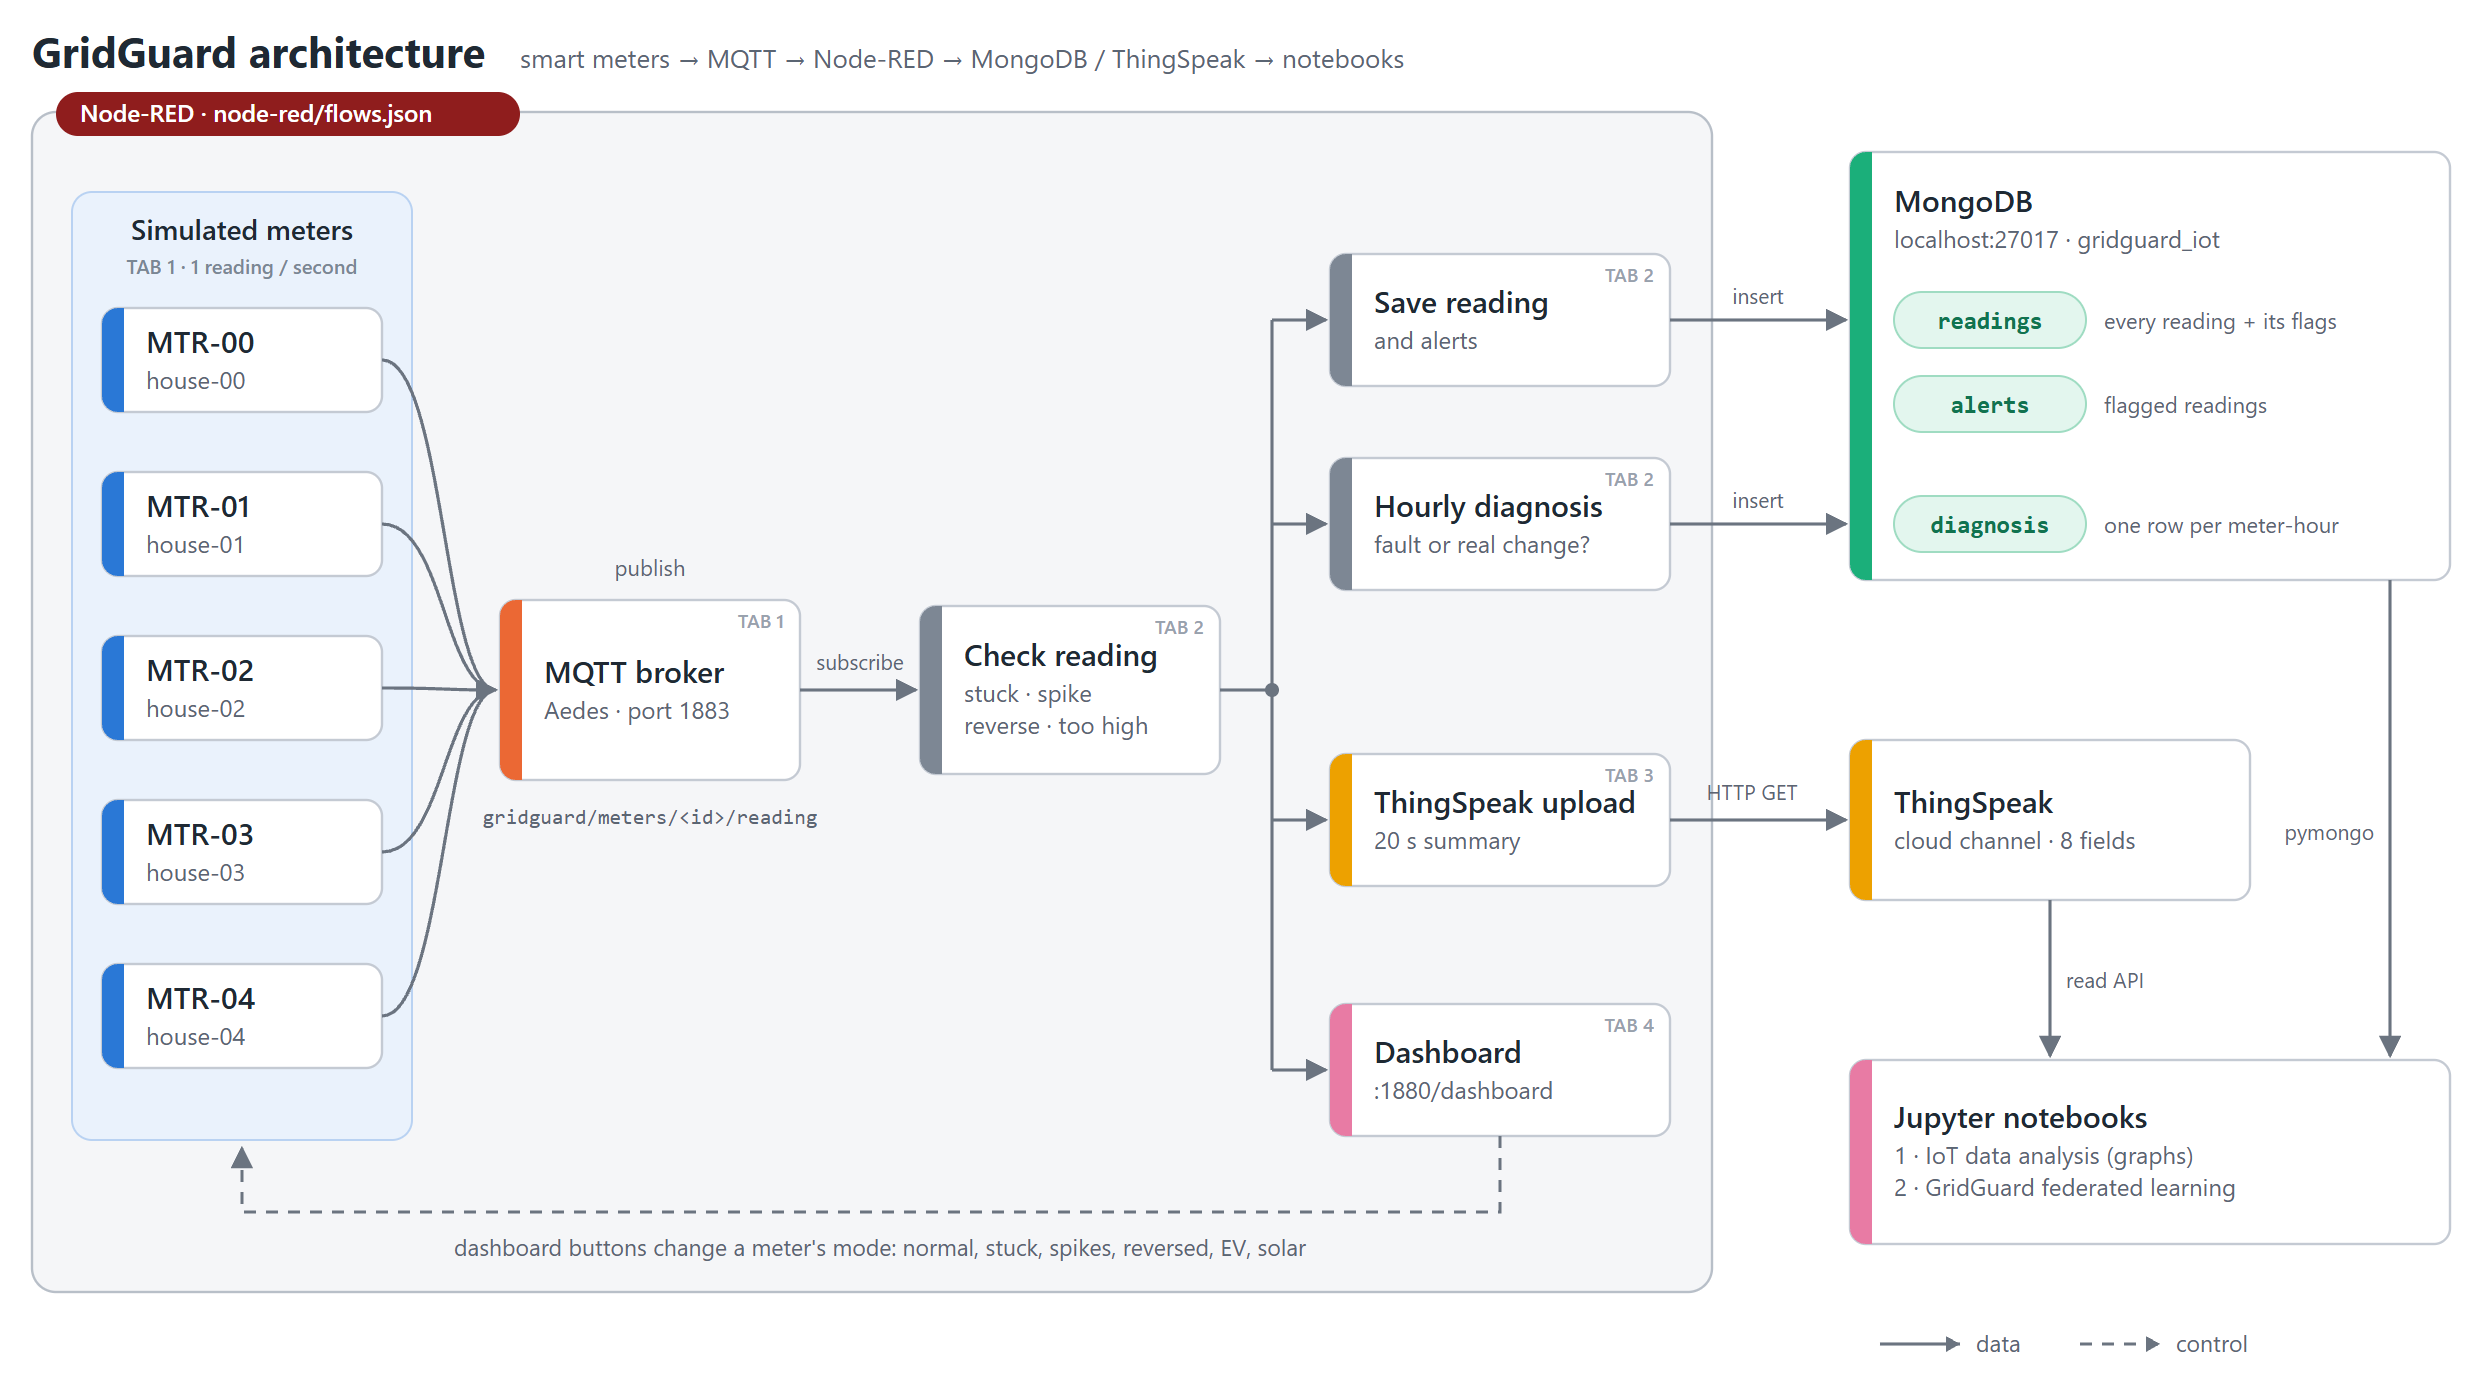
\includegraphics[width=\textwidth]{architecture.png}
\caption{GridGuard architecture. Solid arrows carry data; the dashed arrow is the control path used to inject faults.}
\label{fig:arch}
\end{figure}

The Node-RED application is split into four tabs (flows):

\begin{enumerate}
\item \textbf{Smart meters:} the MQTT broker, the meter simulator, and an MQTT listener for control commands.
\item \textbf{Ingest, detect, store:} subscribes to the readings, checks them, diagnoses every hour and writes to MongoDB.
\item \textbf{ThingSpeak:} averages the data over 20-second windows and uploads it over HTTP.
\item \textbf{Dashboard:} all user-interface widgets.
\end{enumerate}

The tabs pass messages to each other through Node-RED link nodes.

\subsection{Message flow}

Figure~\ref{fig:seq} is a UML sequence diagram of one reading travelling through the system, and of a control command sent back from the dashboard. Table~\ref{tab:topics} lists the MQTT topics.

\begin{figure}[H]
\centering
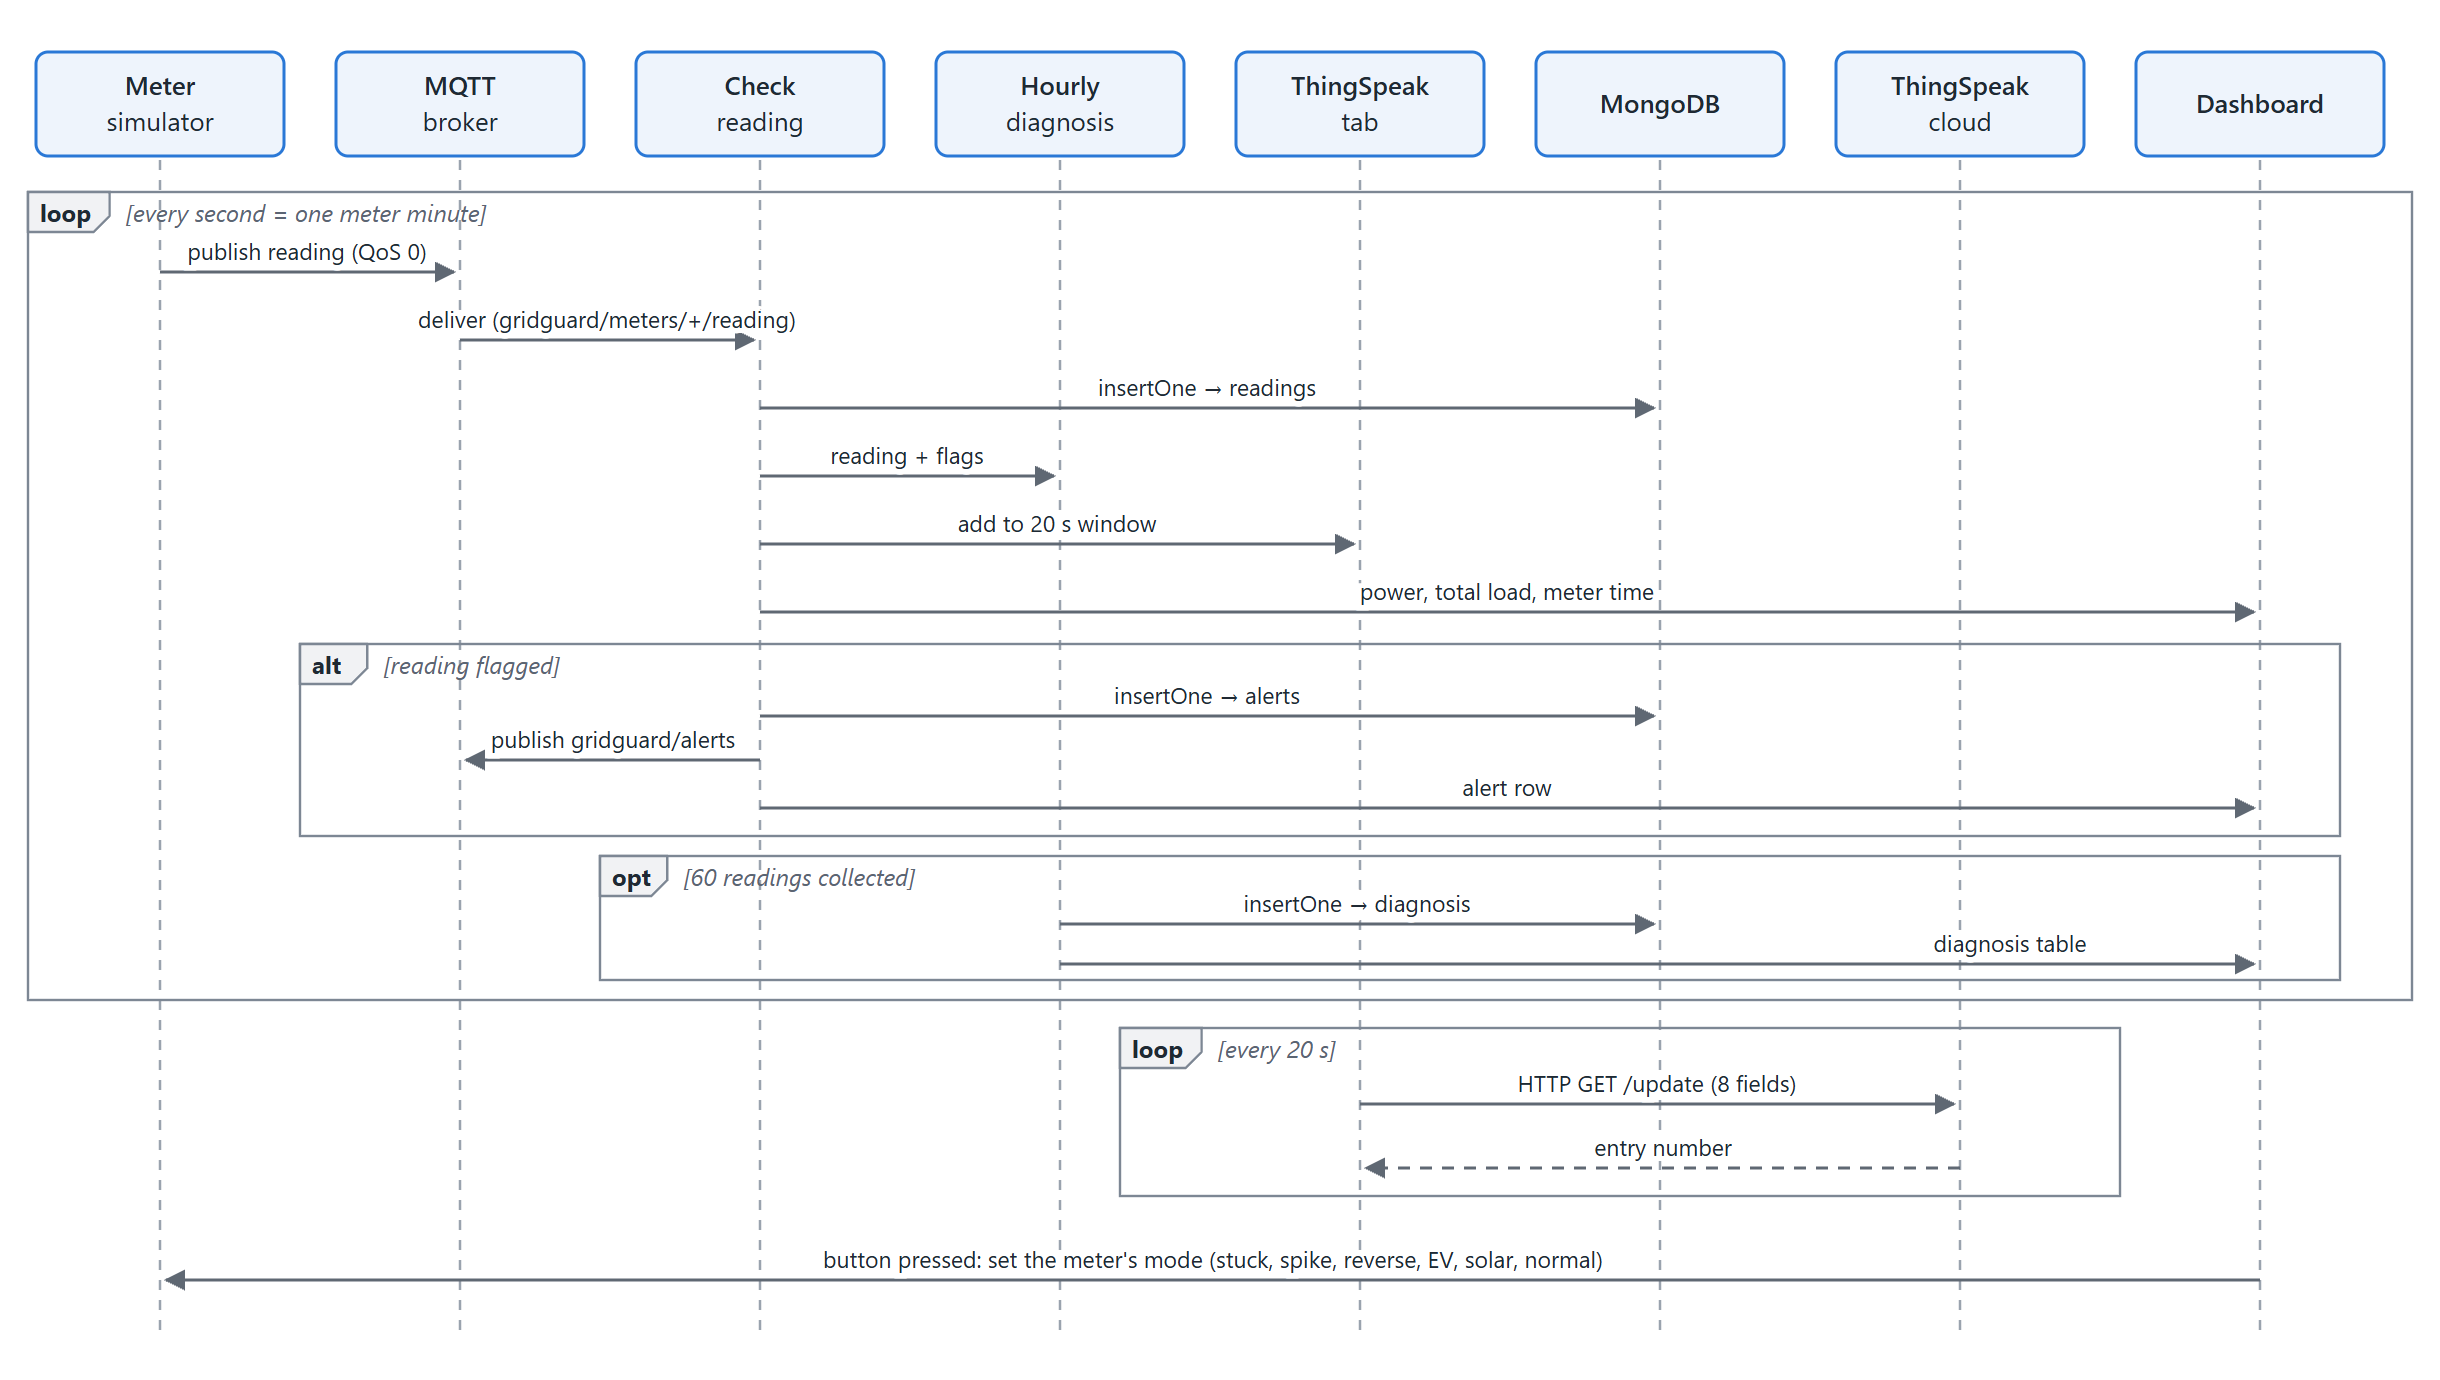
\includegraphics[width=\textwidth]{uml_sequence.png}
\caption{UML sequence diagram: one reading, the optional alert and diagnosis, the ThingSpeak upload and a control command}
\label{fig:seq}
\end{figure}

\begin{table}[H]
\centering
\caption{MQTT topics}
\label{tab:topics}
\small
\begin{tabularx}{\textwidth}{>{\ttfamily\raggedright\arraybackslash}p{6.1cm} c L}
\toprule
\textbf{\rmfamily Topic} & \textbf{QoS} & \textbf{Content}\\
\midrule
gridguard/meters/<id>/reading & 0 & one reading: meter\_id, household\_id, session, ts, power\_w, voltage\_v \\
gridguard/control/<id> or /all & 1 & \texttt{\{"mode": "stuck"\}}: changes the simulated condition of a meter \\
gridguard/alerts & 1 & every flagged reading \\
\bottomrule
\end{tabularx}
\end{table}

Readings use QoS 0 (at most once): a new reading arrives every second, so a lost reading costs little. Commands and alerts use QoS 1 (at least once), because losing one of them would change the behaviour of the system.

\subsection{Smart-meter simulation}

The \emph{Simulate 5 meters} function runs once per second. One second of real time is one minute of meter time, so a full day takes 24 minutes. The meter clock starts at midnight. Every home is built from the same appliance models, with different sizes (Table~\ref{tab:sim}). The function then applies the home's current \emph{mode} (Table~\ref{tab:modes}).

\begin{table}[H]
\centering
\caption{Household load model (home index $i = 0 \dots 4$)}
\label{tab:sim}
\small
\begin{tabularx}{\textwidth}{>{\raggedright\arraybackslash}p{3.3cm} L}
\toprule
\textbf{Component} & \textbf{Model}\\
\midrule
Standby load & $50 + 25i$~W with a $\pm 5\%$ daily variation \\
Morning load & $+(60 + 20i)$~W from 06:30 to 08:30 \\
Evening load & $+(120 + 40i)$~W from 17:30 to 23:00 \\
Fridge & $85 + 10i$~W, on for 15--22 minutes, off for 30--45 minutes \\
Kettle & 2500~W for 3 minutes, started with probability 1.2\% per minute in the morning and evening \\
Washing machine & 65-minute cycle: 2000~W heating, 220~W washing, 500~W spinning (rare, daytime only) \\
Noise and voltage & $\pm 2$~W noise; voltage $230 \pm 2$~V \\
\bottomrule
\end{tabularx}
\end{table}

\begin{table}[H]
\centering
\caption{Meter modes that can be switched on from the dashboard or over MQTT}
\label{tab:modes}
\small
\begin{tabularx}{\textwidth}{>{\ttfamily}l l L}
\toprule
\textbf{\rmfamily Mode} & \textbf{Type} & \textbf{Effect on the reading}\\
\midrule
normal & -- & none \\
stuck & meter fault & the value freezes at its current level \\
spike & meter fault & 5\% of readings jump by 5--15~kW \\
reverse & meter fault & the sign flips (meter installed backwards) \\
ev & genuine change & +7~kW from 19:00 to 23:00 \\
solar & genuine change & $-3000\cdot\max\!\big(0,\sin(\pi(m-390)/720)\big)$~W, where $m$ is the minute of the day (export from 06:30 to 18:30, peak at 12:30) \\
\bottomrule
\end{tabularx}
\end{table}

\subsection{Real-time validation}

The \emph{Check reading} function (Figure~\ref{fig:check}) receives every reading. It keeps a small state object per meter and holds each reading back by one step, so that a reading can be compared with both its predecessor and its successor. It then applies four rules:

\begin{itemize}
\item \textbf{stuck:} the same value 10 times in a row. Real readings always vary slightly.
\item \textbf{spike:} more than 4~kW above both neighbours. No household appliance switches on and off within one minute.
\item \textbf{reverse:} below $-20$~W between 00:00 and 04:00. Solar panels cannot export at night.
\item \textbf{implausible:} more than 23~kW, which is more than a household supply can deliver.
\end{itemize}

The reading is stored with its list of flags. A flagged reading also produces an alert.

\begin{figure}[H]
\centering
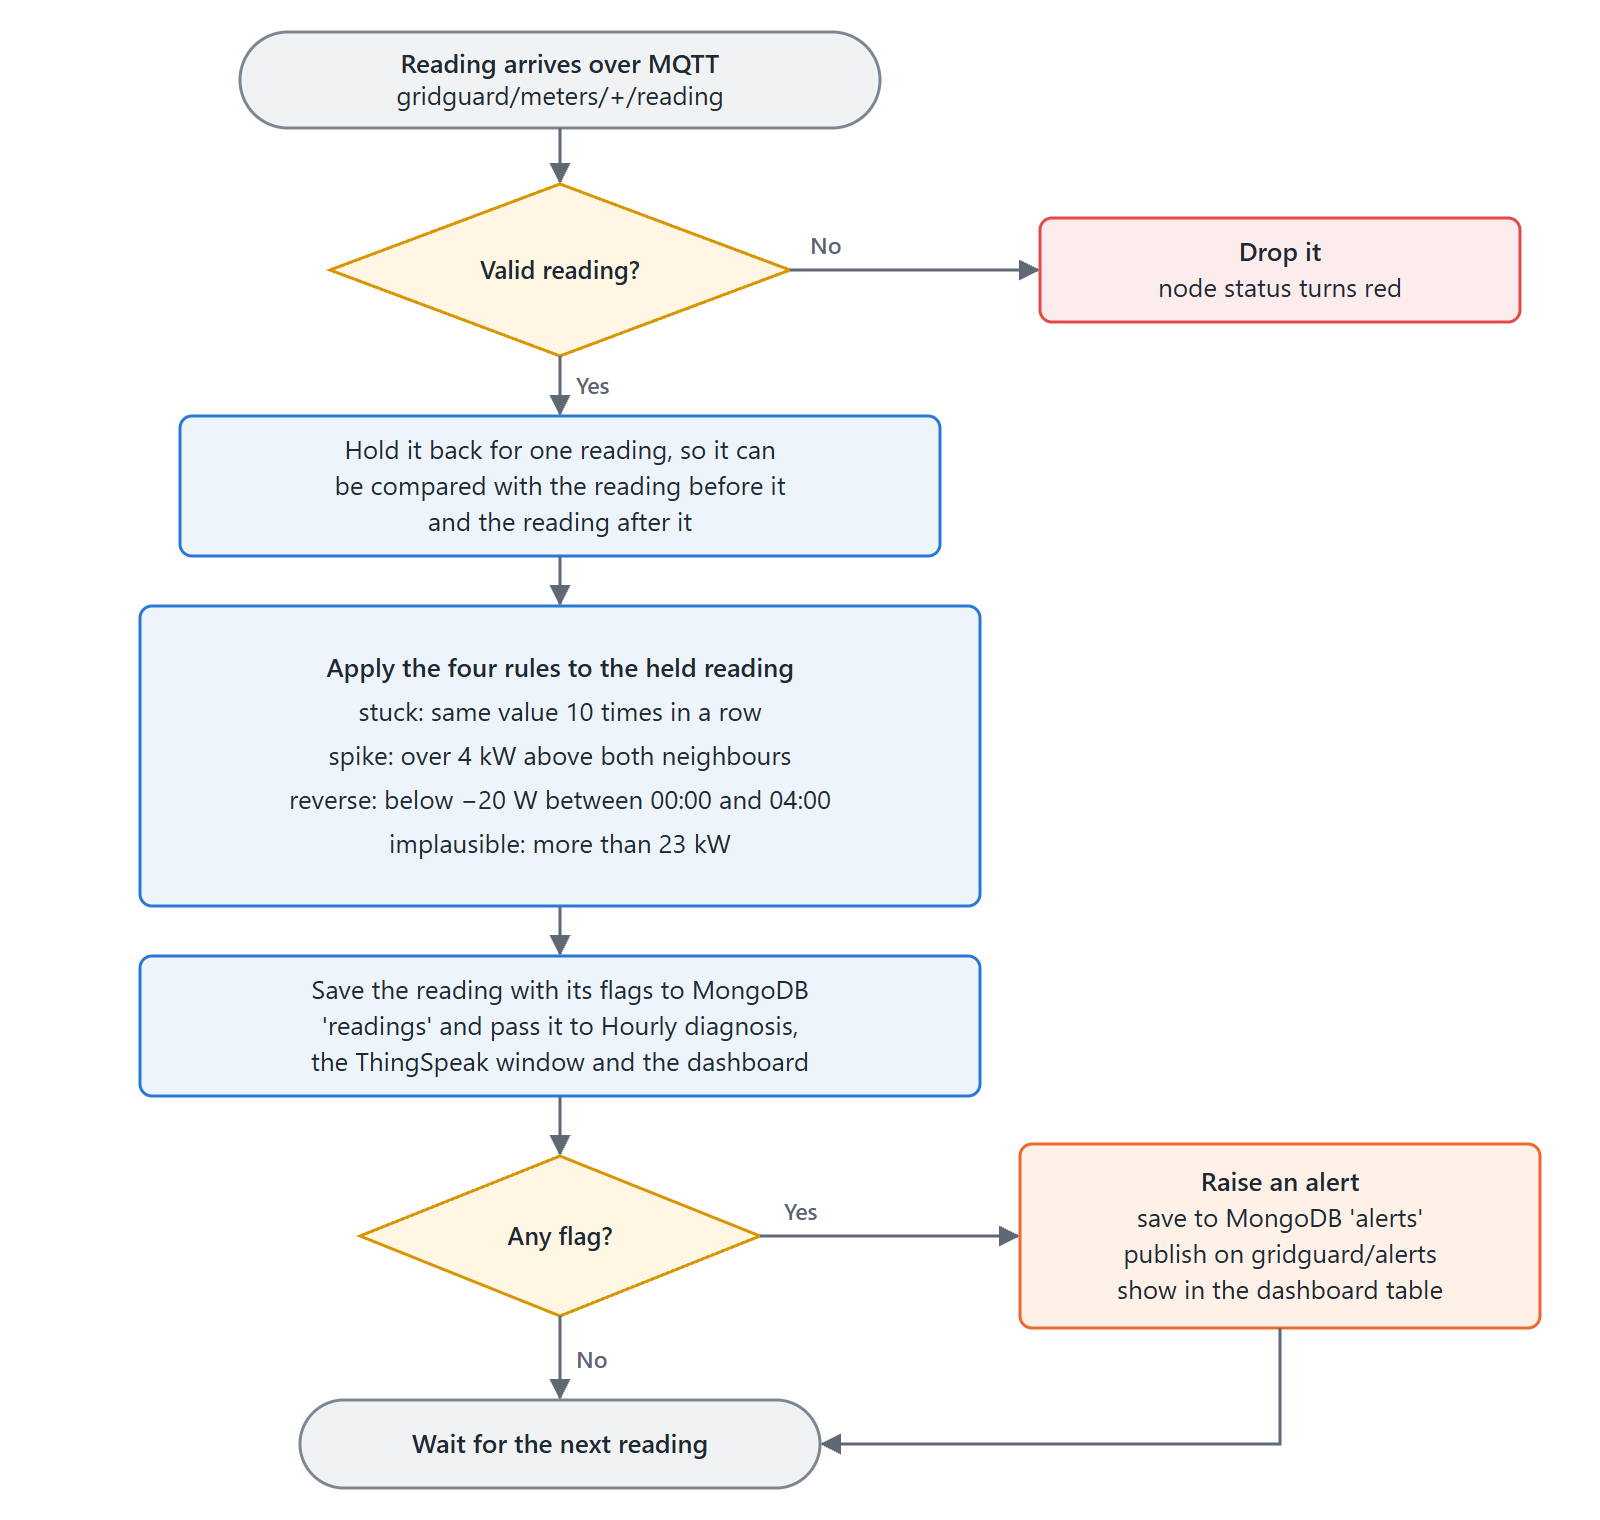
\includegraphics[width=0.78\textwidth]{flow_check_reading.png}
\caption{Flowchart of the \emph{Check reading} function}
\label{fig:check}
\end{figure}

\subsection{Hourly edge diagnosis}

The \emph{Hourly diagnosis} function (Figure~\ref{fig:diag}) is where the GridGuard idea runs at the edge. It buffers 60 readings (one meter-hour) per meter and summarises them:

\begin{itemize}
\item the share of frozen readings;
\item the number of spikes;
\item the share of negative readings;
\item the number of minutes above 5~kW.
\end{itemize}

During daylight, a reversed meter and a solar home look the same, because both read negative. The difference appears after sunset: solar stops exporting, but a reversed meter stays negative. The function therefore remembers, for every meter, whether it was mostly negative while the sun was down (19:00 to 06:00). It uses that memory to label a negative daytime hour as \emph{meter fault} for a meter that was negative at night, and as \emph{genuine change} otherwise.

\begin{figure}[H]
\centering
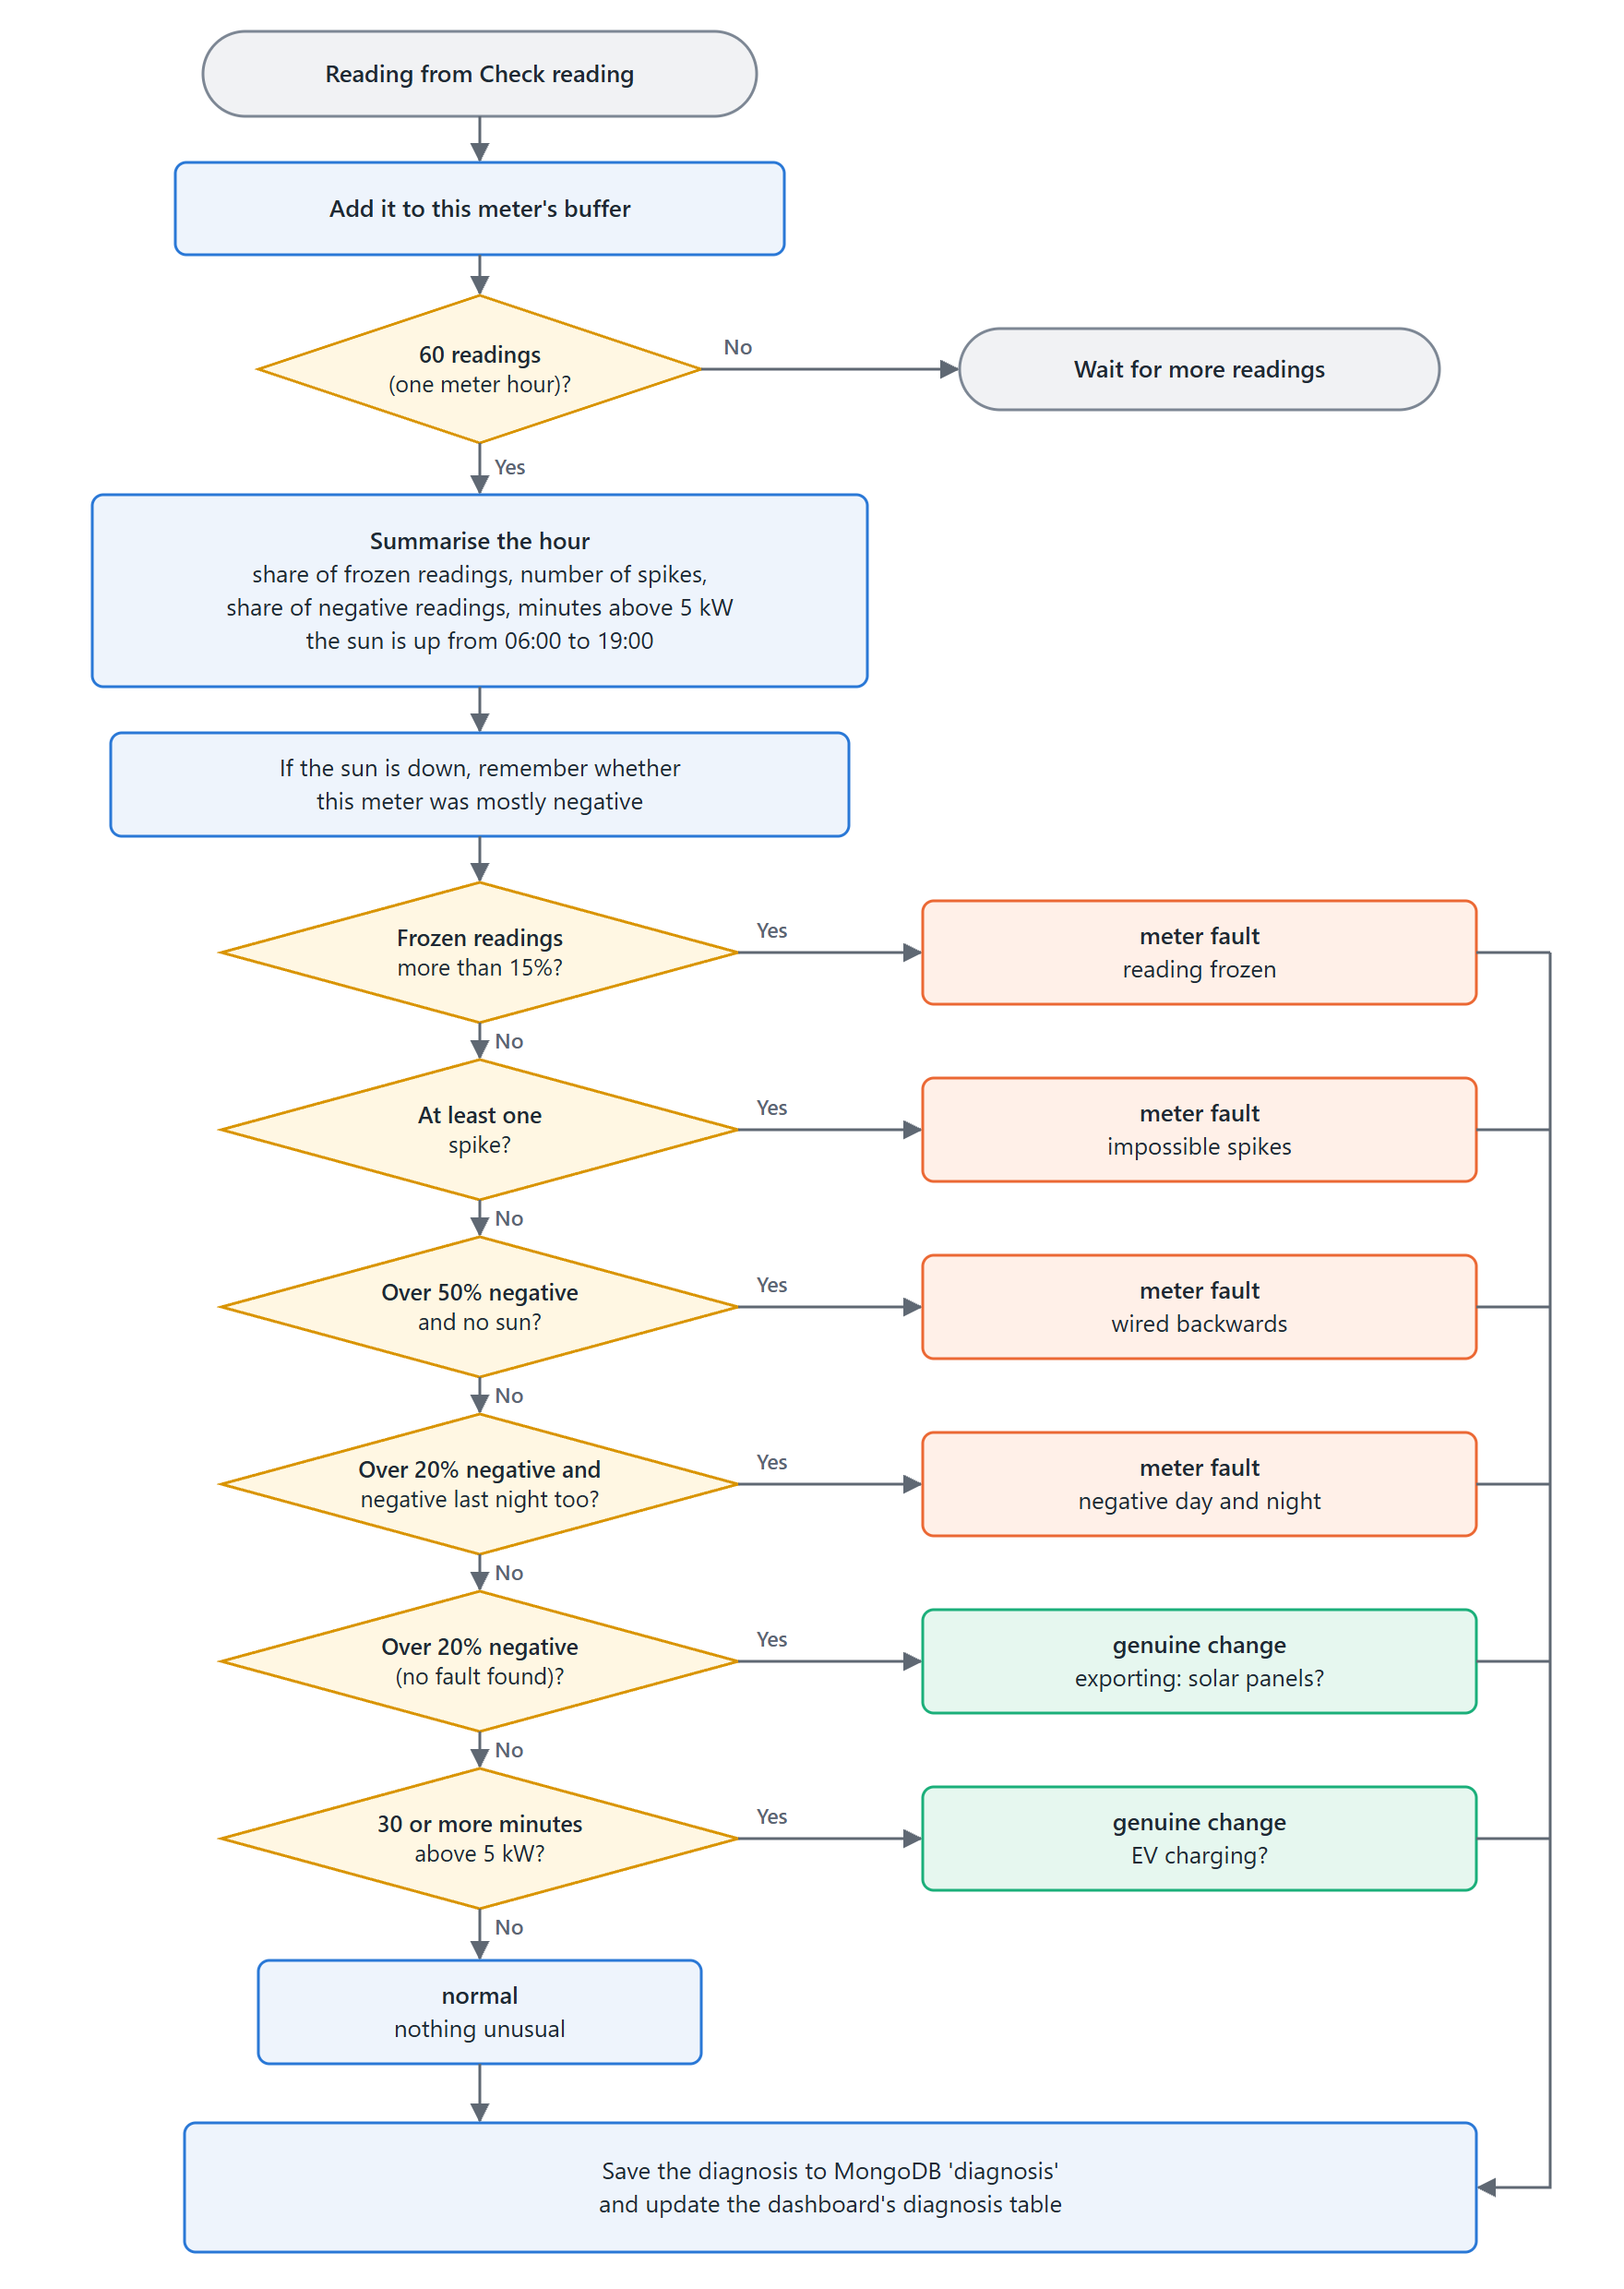
\includegraphics[width=0.74\textwidth]{flow_hourly_diagnosis.png}
\caption{Flowchart of the \emph{Hourly diagnosis} function. The checks run top to bottom and the first match decides.}
\label{fig:diag}
\end{figure}

\subsection{Data storage design}

MongoDB is a document database, so every message is stored directly as a JSON document without a fixed table schema. Node-RED writes to three collections in the database \texttt{gridguard\_iot}, using the \texttt{insertOne} operation of the \texttt{node-red-contrib-mongodb4} node. Every document carries the \texttt{session} in which it was produced, so separate runs can be analysed separately. Figure~\ref{fig:classes} shows the document structure, together with the Python classes used in notebook 2.

\begin{figure}[H]
\centering
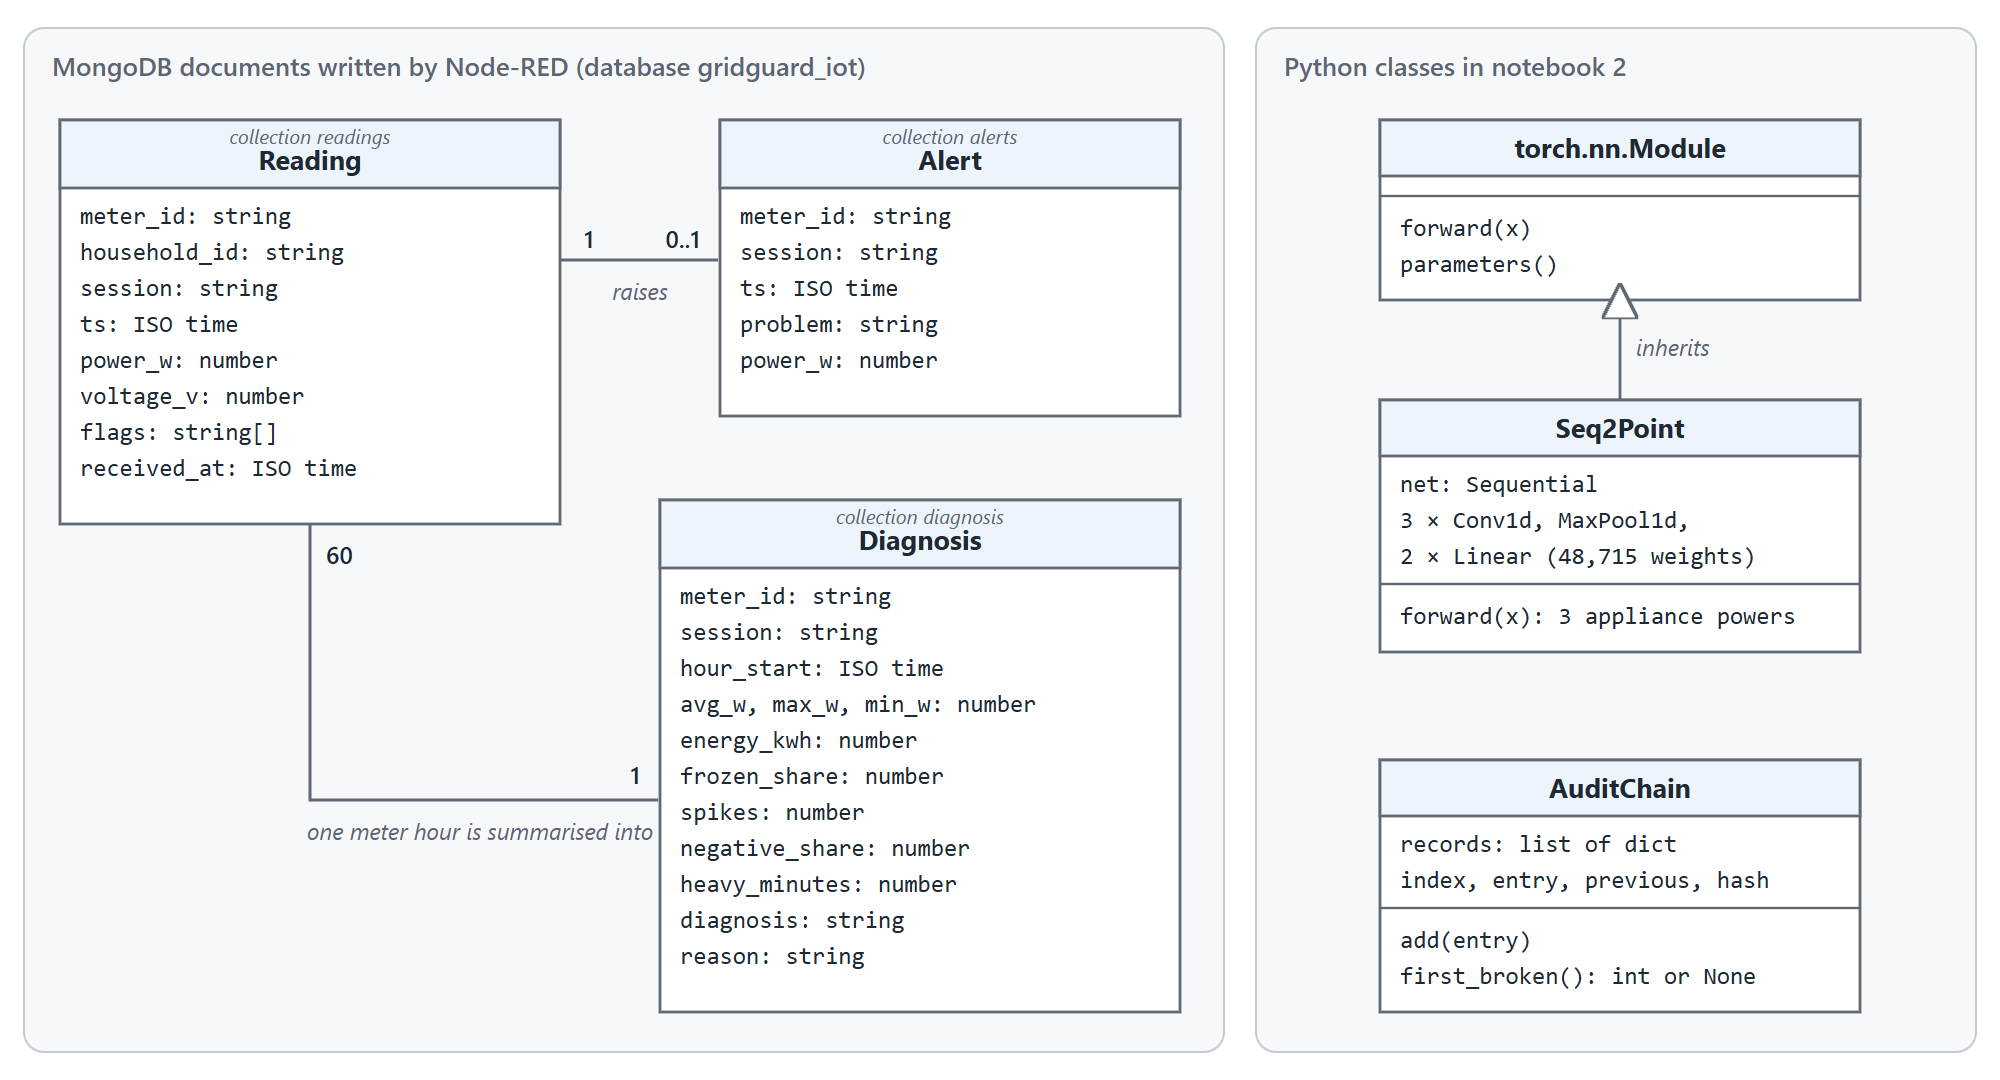
\includegraphics[width=\textwidth]{uml_classes.png}
\caption{UML class diagram: MongoDB documents and Python classes}
\label{fig:classes}
\end{figure}

\subsection{Cloud upload to ThingSpeak}

The ThingSpeak flow collects every checked reading into a 20-second window. Every 20 seconds it sends one HTTP GET request to \texttt{https://api.thingspeak.com/update} with the channel's Write API key and the eight fields in Table~\ref{tab:fields}. The free plan accepts at most one update every 15 seconds, so 20 seconds leaves a safety margin. The key is read from the tab's environment variable \texttt{THINGSPEAK\_WRITE\_KEY}. If the key is missing, the node shows a grey status and sends nothing. A \emph{Check response} node shows the entry number returned by ThingSpeak, or the error if the request was refused.

\begin{table}[H]
\centering
\caption{ThingSpeak channel fields}
\label{tab:fields}
\small
\begin{tabular}{ll}
\toprule
\textbf{Field} & \textbf{Value over the last 20 seconds}\\
\midrule
field1 -- field5 & average power of MTR-00 to MTR-04 (W) \\
field6 & total neighbourhood load (W) \\
field7 & number of flagged readings \\
field8 & number of meters with at least one flagged reading \\
\bottomrule
\end{tabular}
\end{table}

\subsection{Dashboard}

The dashboard (FlowFuse Node-RED Dashboard 2.0, at \texttt{/dashboard/gridguard}) shows:

\begin{itemize}
\item a live line chart of the last 3 minutes of every meter;
\item a gauge of the total load (green below 8~kW, orange up to 15~kW, red above);
\item the meter clock;
\item a meter selector with six buttons (Normal, Stuck, Spikes, Reversed, EV charger, Solar) to change the selected meter's mode;
\item the latest diagnosis of every meter, with its reason;
\item the last 12 alerts.
\end{itemize}

\subsection{Federated learning with GridGuard}

\textbf{NILM model.} The Sequence-to-Point network \cite{s2p} receives a window of 59 minutes of aggregate power and predicts the power of the fridge, the kettle and the washing machine at the middle minute. It has three 1-D convolution layers, one max-pooling layer and two fully connected layers, 48,715 parameters in total. The model is implemented as the class \texttt{Seq2Point}, which inherits from \texttt{torch.nn.Module}.

\textbf{Homes and data.} Eight homes are simulated for 11 days at one-minute resolution, including the true power of each appliance. The first three days are a warm-up history. Two further homes, which never take part in training, are used to measure the error in watts (mean absolute error).

\textbf{FedAvg.} In round $t$ every home $k$ starts from the global weights $w^t$ and trains for 2 epochs on its last two days of data (Adam optimiser, learning rate $10^{-3}$, batch size 128). It sends the update $\Delta_k = w_k - w^t$, and the server averages the updates weighted by the number of training samples $n_k$:
\begin{equation}
w^{t+1} = w^t + \frac{\sum_k n_k \Delta_k}{\sum_k n_k}
\end{equation}

\textbf{Threat and fault model.} From round 3 or later, the following events are switched on:

\begin{itemize}
\item \textbf{attacks:}
  \begin{itemize}
  \item sign flip: the home sends $-5\Delta_k$;
  \item scaling: the home sends $20\Delta_k$;
  \item tampering: the update is changed in transit, after it was signed;
  \end{itemize}
\item \textbf{meter faults:} stuck and reversed meters;
\item \textbf{genuine changes:} an EV charger and solar panels.
\end{itemize}

\textbf{Evidence.} GridGuard collects two kinds of evidence:

\begin{itemize}
\item \textbf{Meter evidence:} six numbers computed inside the home from its readings:
  \begin{itemize}
  \item the share of spikes;
  \item the share of stuck readings;
  \item the negative share at night;
  \item the negative share in daylight;
  \item the logarithmic change in average usage compared with the home's history;
  \item the share of hours above 5~kW.
  \end{itemize}
  These are the same ideas Node-RED applies in Sections 2.1.4 and 2.1.5.
\item \textbf{Update evidence:} computed by the server:
  \begin{itemize}
  \item size: $s_k = \lVert\Delta_k\rVert / \operatorname{median}_j \lVert\Delta_j\rVert$;
  \item direction: $d_k = \cos(\Delta_k, \operatorname{median}_{j\neq k}\Delta_j)$, the cosine similarity with the coordinate-wise median of the other updates.
  \end{itemize}
\end{itemize}

\textbf{Cause attribution.} The meter is examined first, because a broken meter also produces an unusual update, and that is not the family's fault.
\begin{itemize}
\item \emph{meter fault} if spikes $> 0.1\%$, stuck $> 5\%$ or negative at night $> 30\%$;
\item otherwise, if the update is odd ($s_k > 3$, or $d_k < 0$, or low integrity with $d_k < 0.1$): \emph{uncertain} if there is also evidence of a real change, and \emph{malicious} if there is not;
\item otherwise \emph{genuine change} if there is evidence of solar export, EV-size load or a large usage shift, and \emph{benign} if there is not.
\end{itemize}

\textbf{Trust and aggregation.} Every home has three scores between 0 and 1:
\begin{itemize}
\item \emph{integrity}, which halves after every attack or bad signature;
\item \emph{reliability}, which is multiplied by 0.6 after every meter fault;
\item \emph{adaptability}, which grows by 0.1 with every confirmed genuine change.
\end{itemize}
A benign update gets weight $\omega_k = I_k$. A genuine change gets $\omega_k = 0.5\,I_k A_k$. Every other cause gets weight 0, and so does any home with $I_k < 0.25$. Every update is first clipped to twice the median size $c$:
\begin{equation}
w^{t+1} = w^t + \frac{\sum_k n_k\,\omega_k\,\tilde\Delta_k}{\sum_k n_k\,\omega_k}, \qquad \tilde\Delta_k = \Delta_k \min\!\left(1, \frac{c}{s_k}\right)
\end{equation}

\textbf{Signatures and audit chain.} Each home owns an Ed25519 key pair \cite{ed25519}. It signs a message containing its id, the round number, the SHA-256 hash \cite{sha} of its update and its meter evidence. The server verifies the signature before looking at anything else, so an update changed in transit is rejected. Every decision is appended to a hash chain \cite{haber}, implemented by the class \texttt{AuditChain}: record $i$ stores $h_i = \text{SHA-256}(i, \text{entry}_i, h_{i-1})$. Editing any old record therefore breaks every hash after it. Figure~\ref{fig:round} summarises one round.

\begin{figure}[H]
\centering
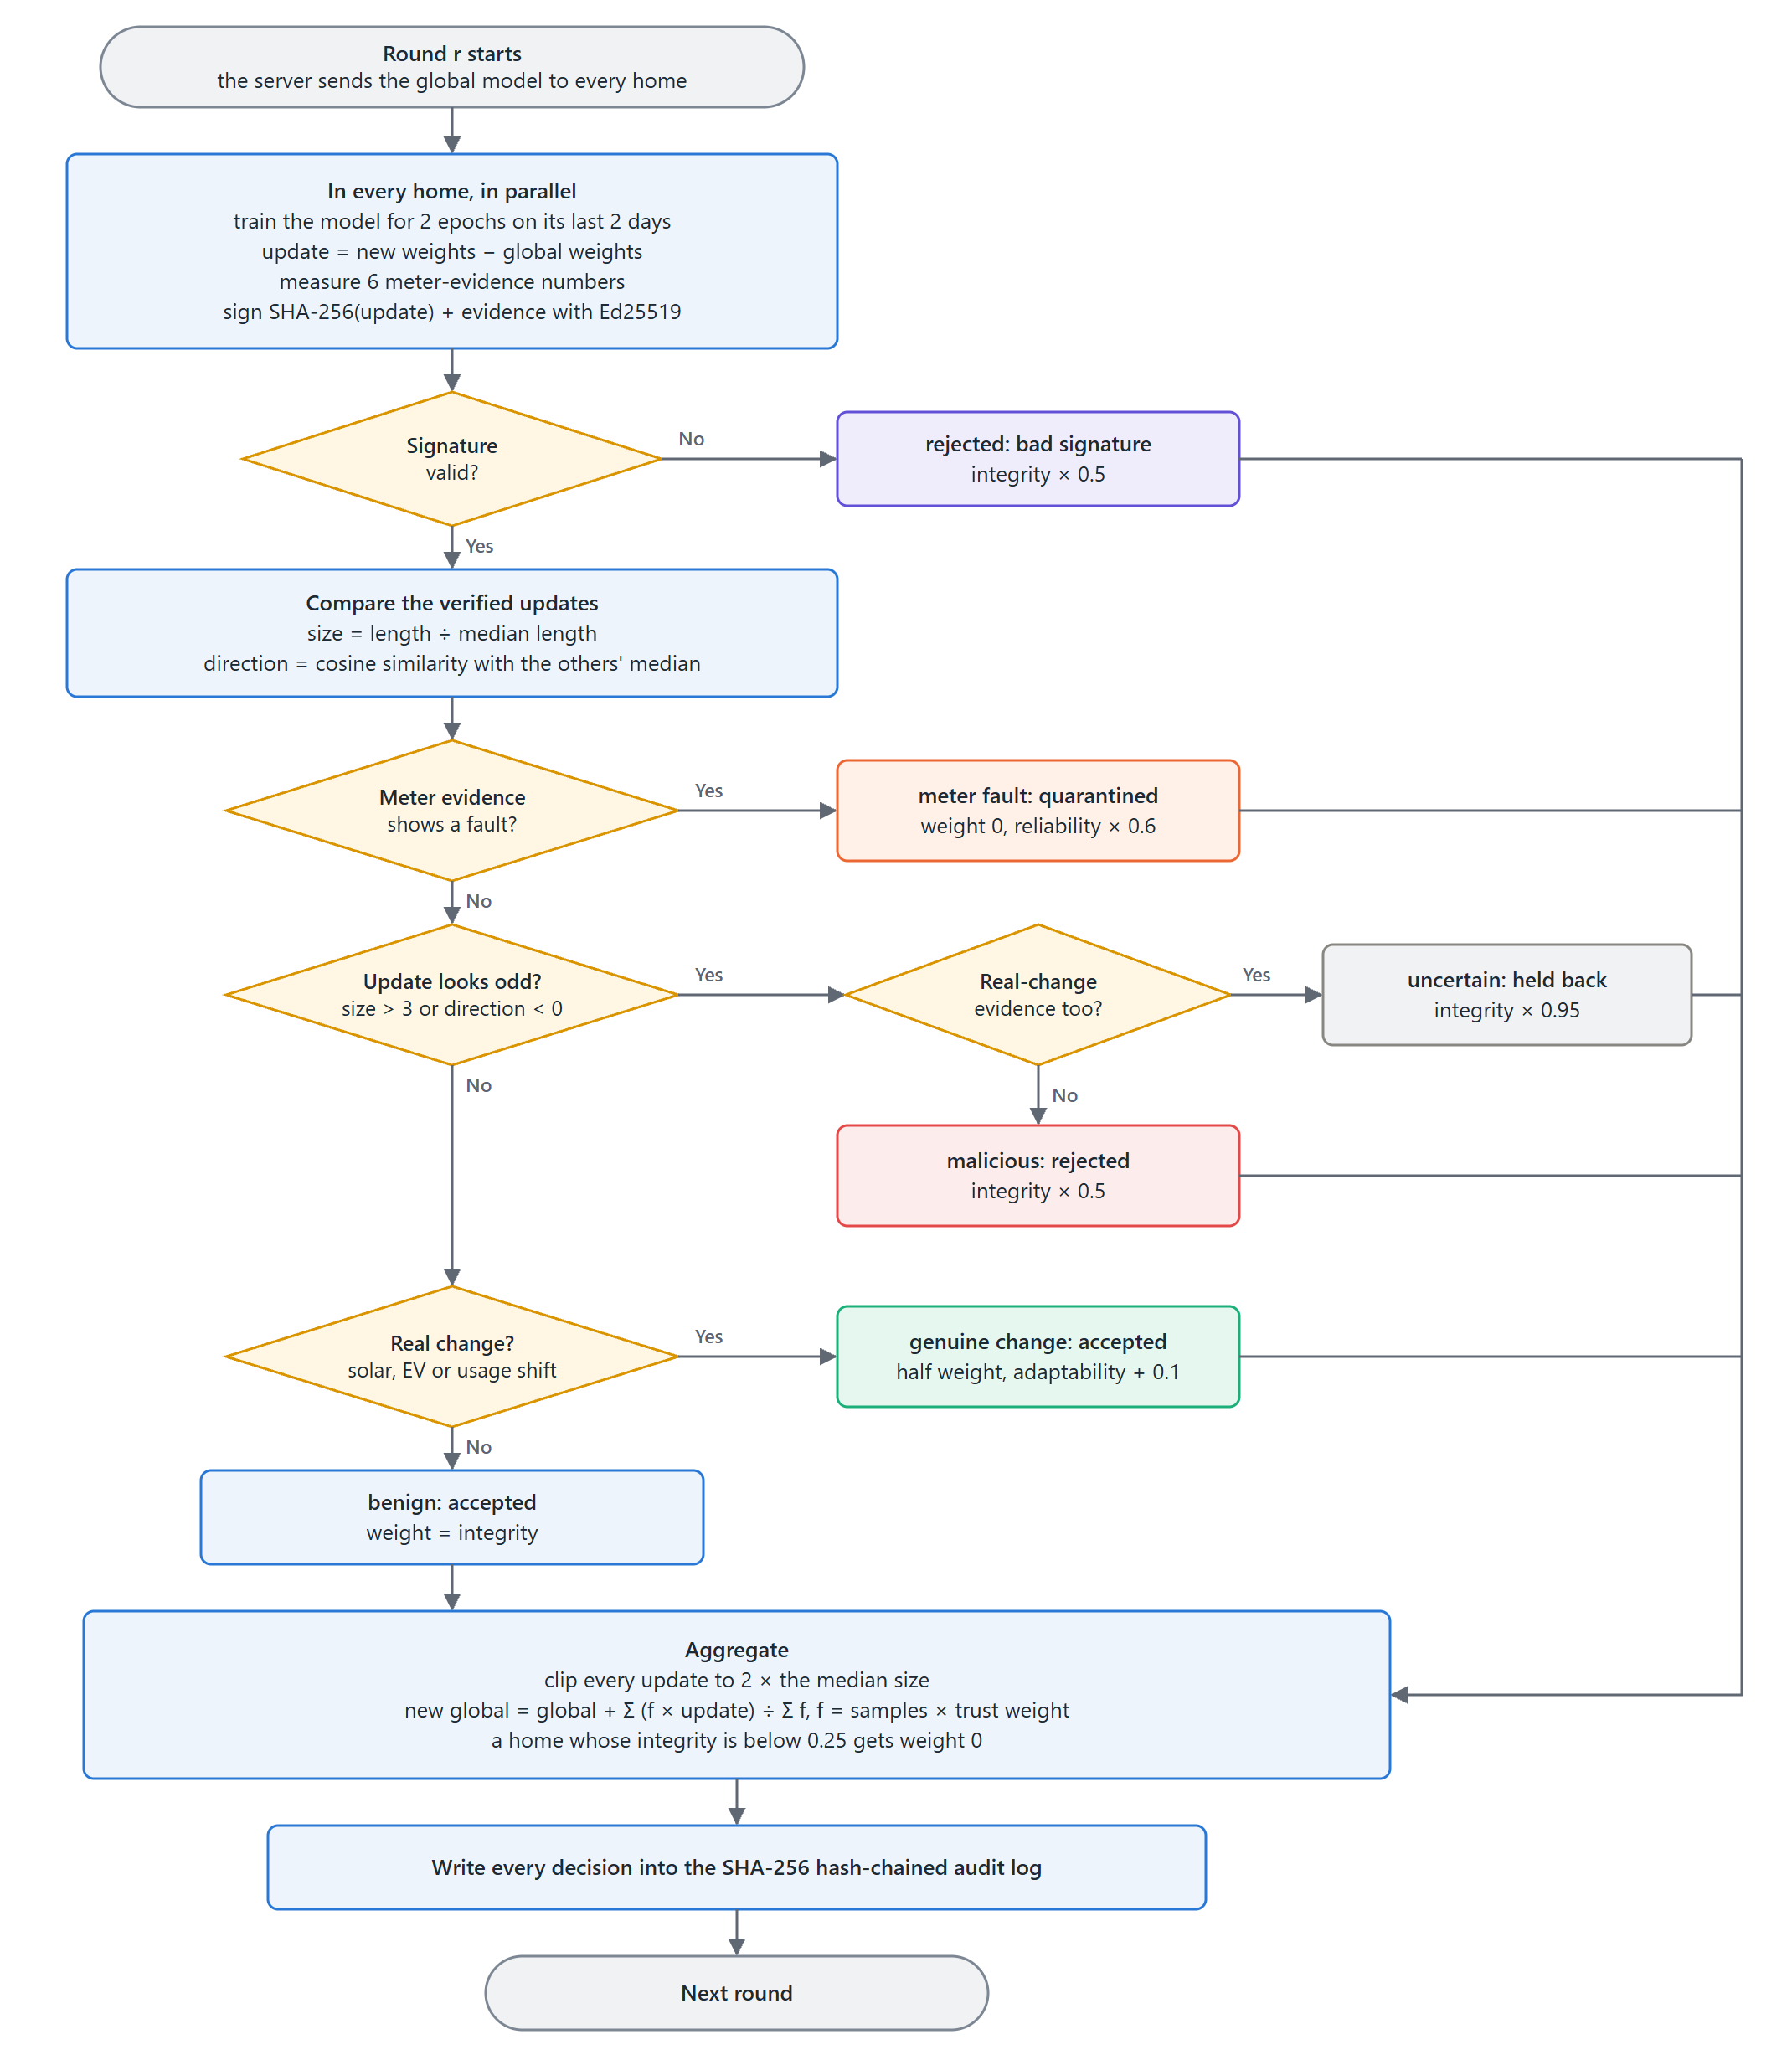
\includegraphics[width=0.9\textwidth]{flow_fl_round.png}
\caption{Flowchart of one GridGuard federated-learning round}
\label{fig:round}
\end{figure}

\chapter{Implementation \& Testing}

\section{Experimental Setup}

\begin{table}[H]
\centering
\caption{Hardware and software used}
\label{tab:setup}
\small
\begin{tabularx}{\textwidth}{>{\raggedright\arraybackslash}p{4.2cm} L}
\toprule
\textbf{Item} & \textbf{Version / details}\\
\midrule
Computer & Laptop, AMD Ryzen 7 7840HS, 16 GB RAM, Windows 11 Home; no GPU used \\
Node.js / Node-RED & Node.js 22.17.0; Node-RED 4.0.9, run locally with \texttt{npm start} \\
Node-RED add-ons & node-red-contrib-aedes 1.4.0 (MQTT broker), node-red-contrib-mongodb4 3.4.0, @flowfuse/node-red-dashboard 1.37.0 \\
Database & MongoDB Community Server 9.0.4 on \texttt{localhost:27017} \\
Cloud & ThingSpeak (free MathWorks account) \\
Python & Python 3.13.5, Jupyter, NumPy 2.5.5, pandas 3.1.1, Matplotlib 3.11.2, PyMongo 4.20.1 \\
Machine learning and security & PyTorch 2.15.0 (CPU), cryptography 50.0.2 (Ed25519) \\
Browser & Microsoft Edge (dashboard and Node-RED editor) \\
\bottomrule
\end{tabularx}
\end{table}

\begin{table}[H]
\centering
\caption{Configuration}
\label{tab:config}
\small
\begin{tabularx}{\textwidth}{>{\raggedright\arraybackslash}p{4.2cm} L}
\toprule
\textbf{Setting} & \textbf{Value}\\
\midrule
Node-RED editor / dashboard & \texttt{http://localhost:1880} and \texttt{/dashboard/gridguard} \\
MQTT broker & Aedes inside Node-RED, port 1883 \\
MongoDB & database \texttt{gridguard\_iot}; collections \texttt{readings}, \texttt{alerts}, \texttt{diagnosis} \\
Simulation speed & 1 real second = 1 meter minute; one day = 24 minutes \\
ThingSpeak & upload every 20 s; Write API key in the tab variable \texttt{THINGSPEAK\_WRITE\_KEY} \\
Federated learning & 8 homes, 8 rounds, 2 local epochs, Adam ($10^{-3}$), batch 128, 59-minute window, 2 unseen test homes \\
\bottomrule
\end{tabularx}
\end{table}

\textbf{Test procedure for the IoT part.} Node-RED was started and one full simulated day was recorded. Faults and changes were switched on with MQTT control messages, which the dashboard buttons also send:
\begin{itemize}
\item MTR-01 was set to \emph{reverse}, MTR-03 to \emph{ev} and MTR-04 to \emph{solar} for the whole day;
\item MTR-02 was set to \emph{stuck} from about 08:13 to 12:13;
\item MTR-00 was set to \emph{spike} from about 14:13 to 16:13.
\end{itemize}
The recorded day starts at 00:13 meter time, because the first readings of that run were sent before Node-RED's MQTT client had connected; the simulator now waits 20 seconds at start-up so that this does not happen again. Notebook 1 then read the session from MongoDB. Notebook 2 runs on its own in about 35 seconds on the CPU.

\section{Results (Test Cases / Screenshots / Output)}

\subsection{Node-RED flows}

Figures~\ref{fig:tab1} and \ref{fig:tab2} show the four flows in the Node-RED editor while the system is running. The small coloured dots under the nodes are live status indicators: \emph{connected} for the MQTT nodes, the meter clock for the simulator, and the number of saved documents for the MongoDB nodes.

\begin{figure}[H]
\centering
\begin{subfigure}{\textwidth}\centering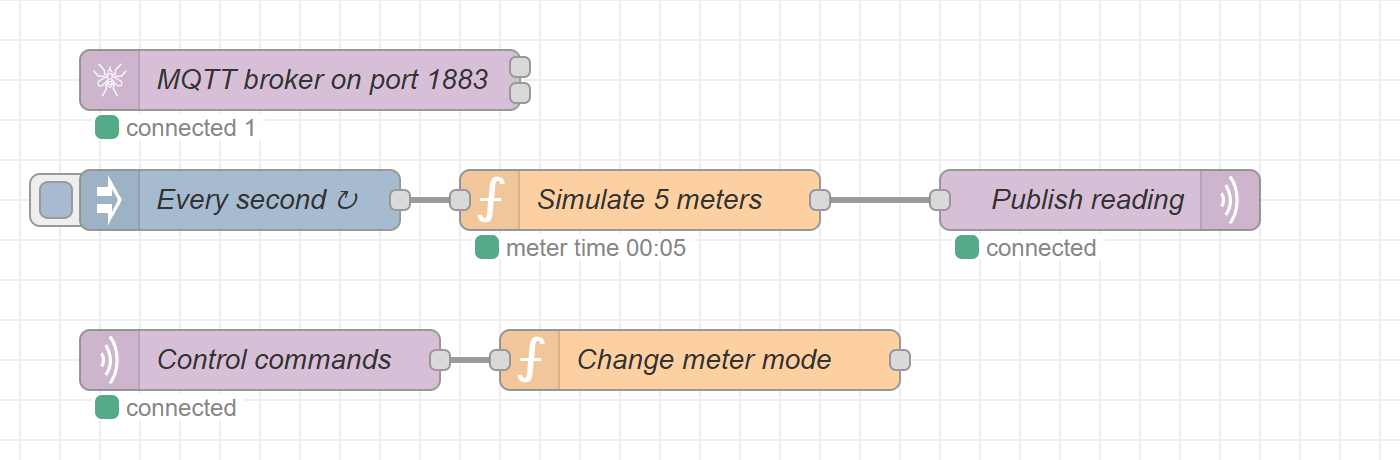
\includegraphics[width=0.62\textwidth]{editor_tab_sim.png}\caption{Tab 1: Smart meters}\end{subfigure}\\[6pt]
\begin{subfigure}{\textwidth}\centering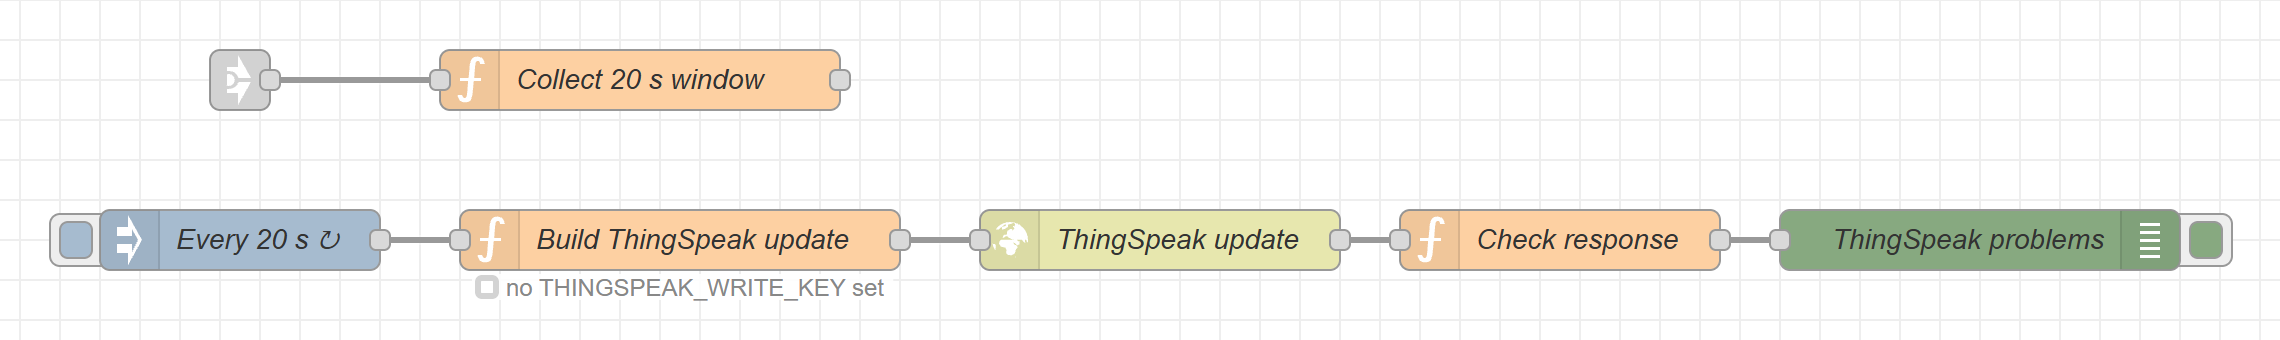
\includegraphics[width=0.95\textwidth]{editor_tab_cloud.png}\caption{Tab 3: ThingSpeak (no key set yet, so the build node shows a grey status)}\end{subfigure}
\caption{Node-RED flows: smart meters and ThingSpeak upload}
\label{fig:tab1}
\end{figure}

\begin{figure}[H]
\centering
\begin{subfigure}{0.56\textwidth}\centering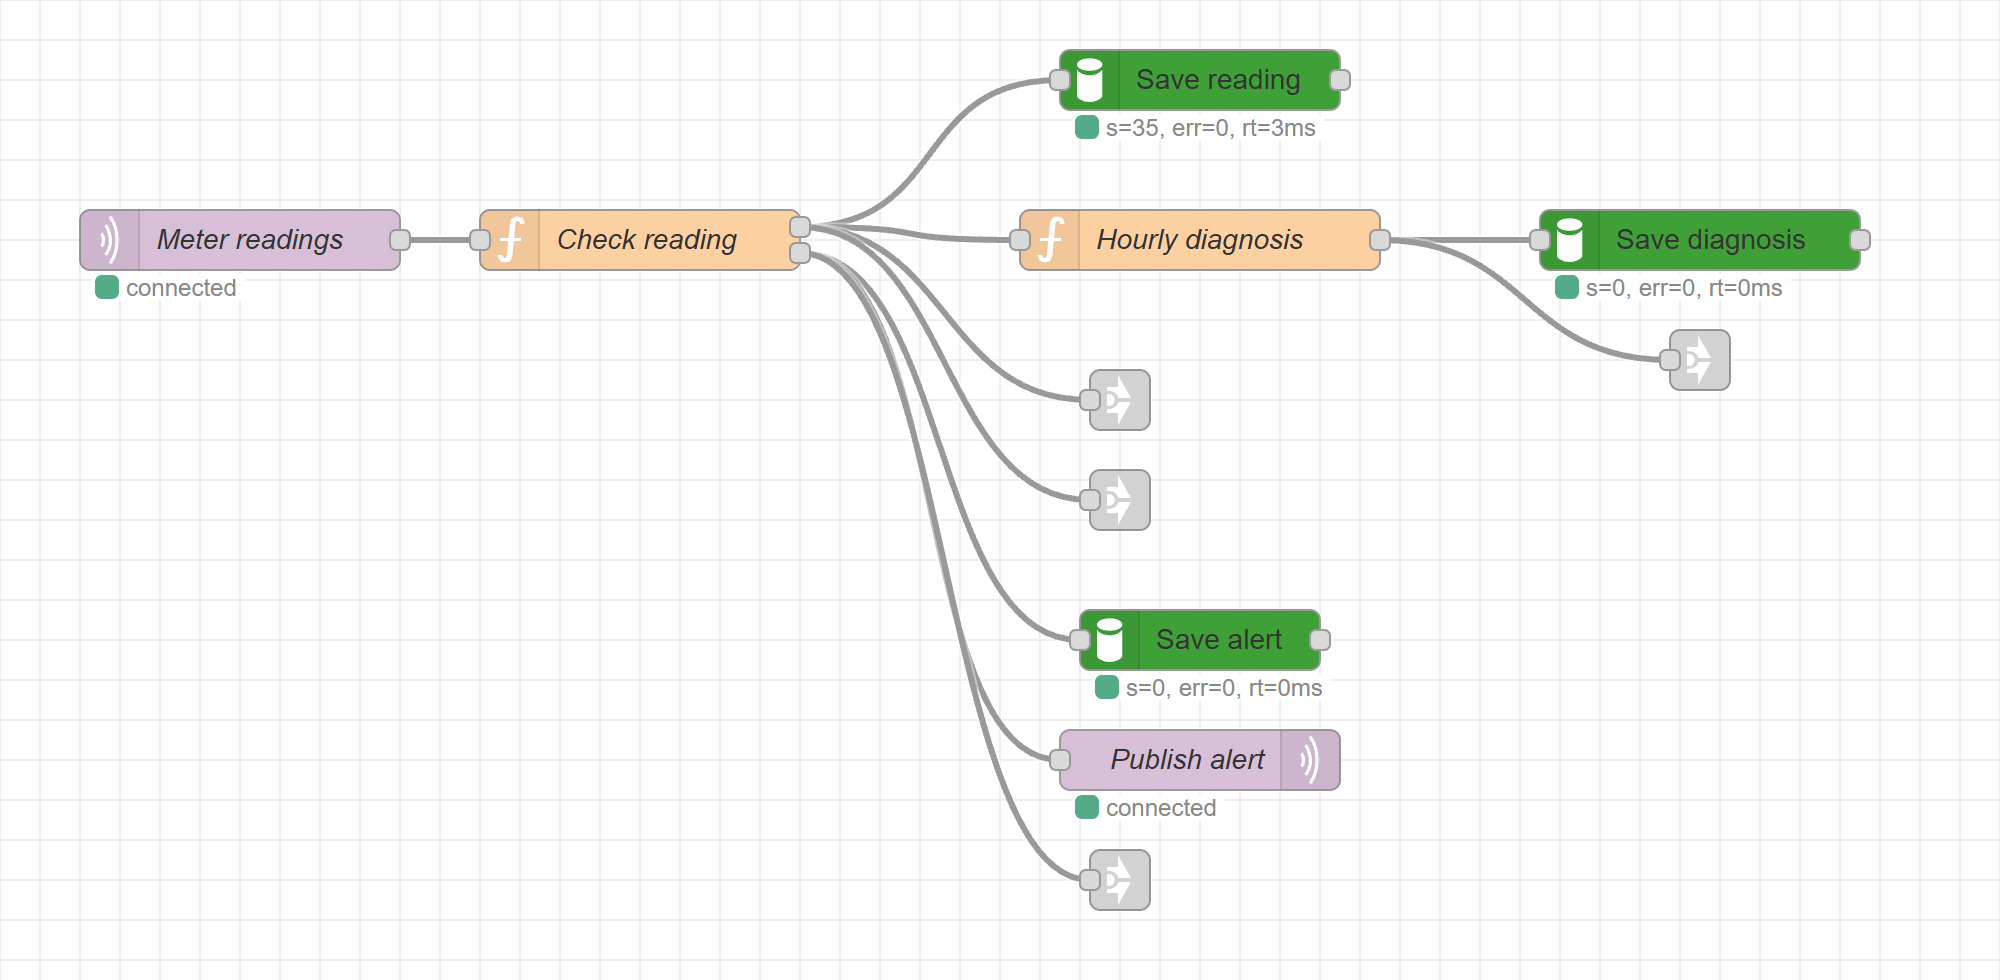
\includegraphics[width=\textwidth]{editor_tab_ingest.png}\caption{Tab 2: Ingest, detect, store}\end{subfigure}\hfill
\begin{subfigure}{0.4\textwidth}\centering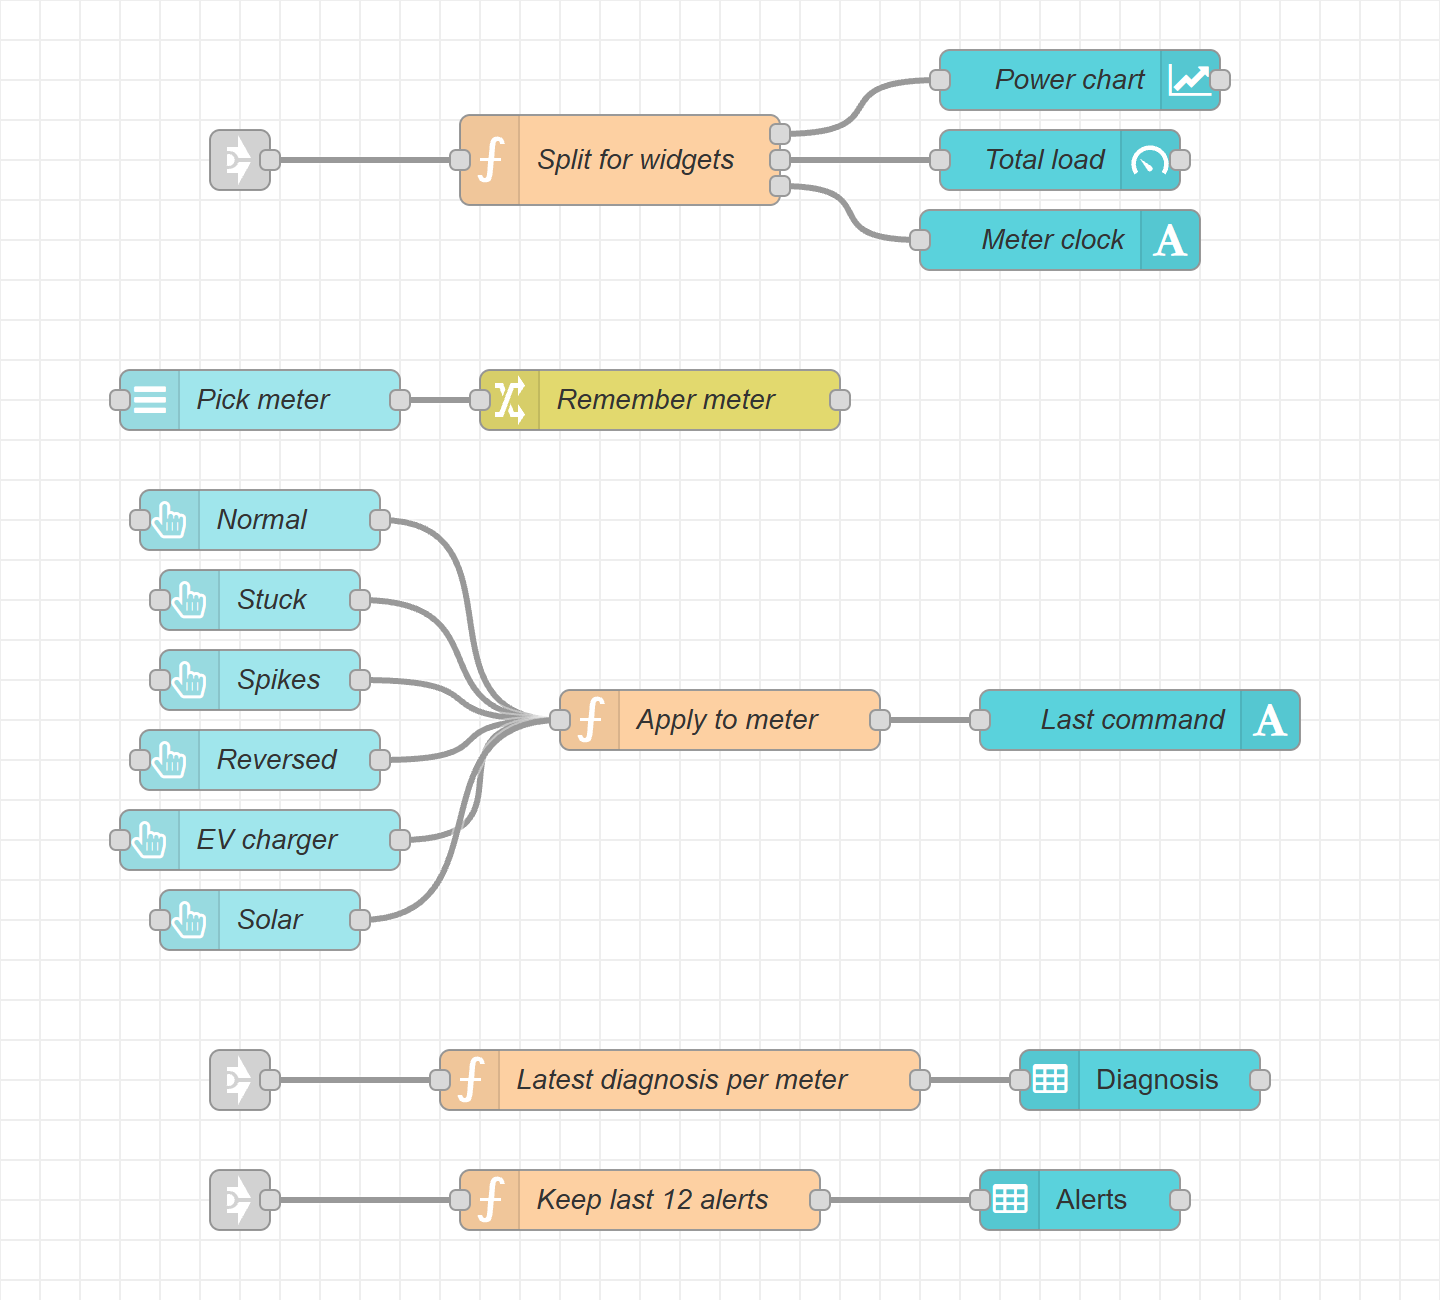
\includegraphics[width=\textwidth]{editor_tab_ui.png}\caption{Tab 4: Dashboard}\end{subfigure}
\caption{Node-RED flows: processing and dashboard}
\label{fig:tab2}
\end{figure}

\subsection{Live dashboard}

\begin{figure}[H]
\centering
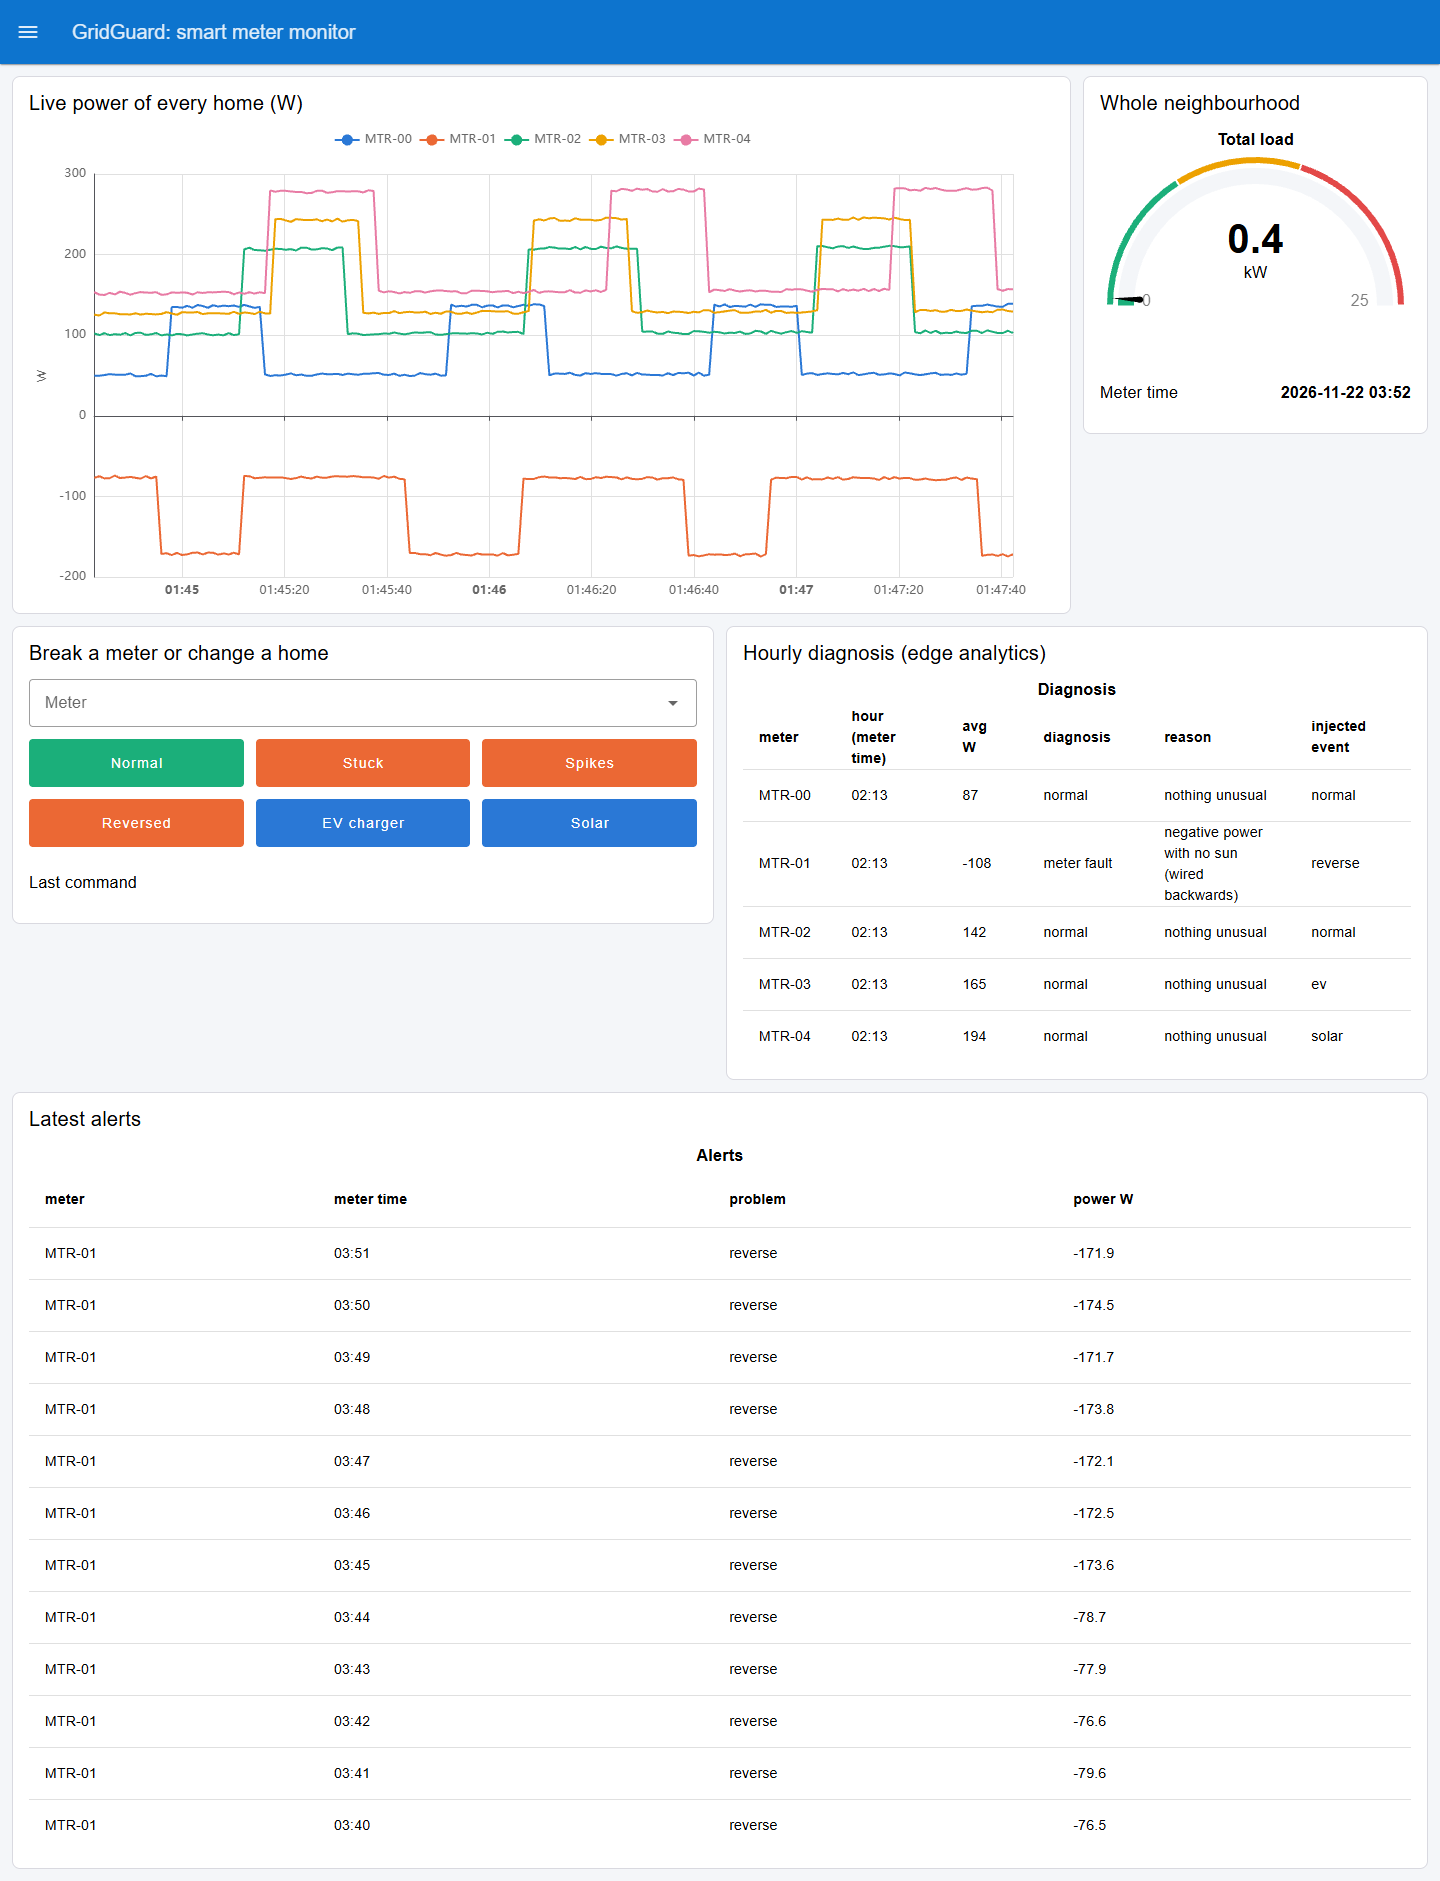
\includegraphics[width=0.9\textwidth]{dashboard-night.png}
\caption{Dashboard at about 03:00 meter time: MTR-01 (reversed) reads negative at night, and its alerts and \emph{meter fault} diagnosis appear}
\label{fig:dash1}
\end{figure}

\begin{figure}[H]
\centering
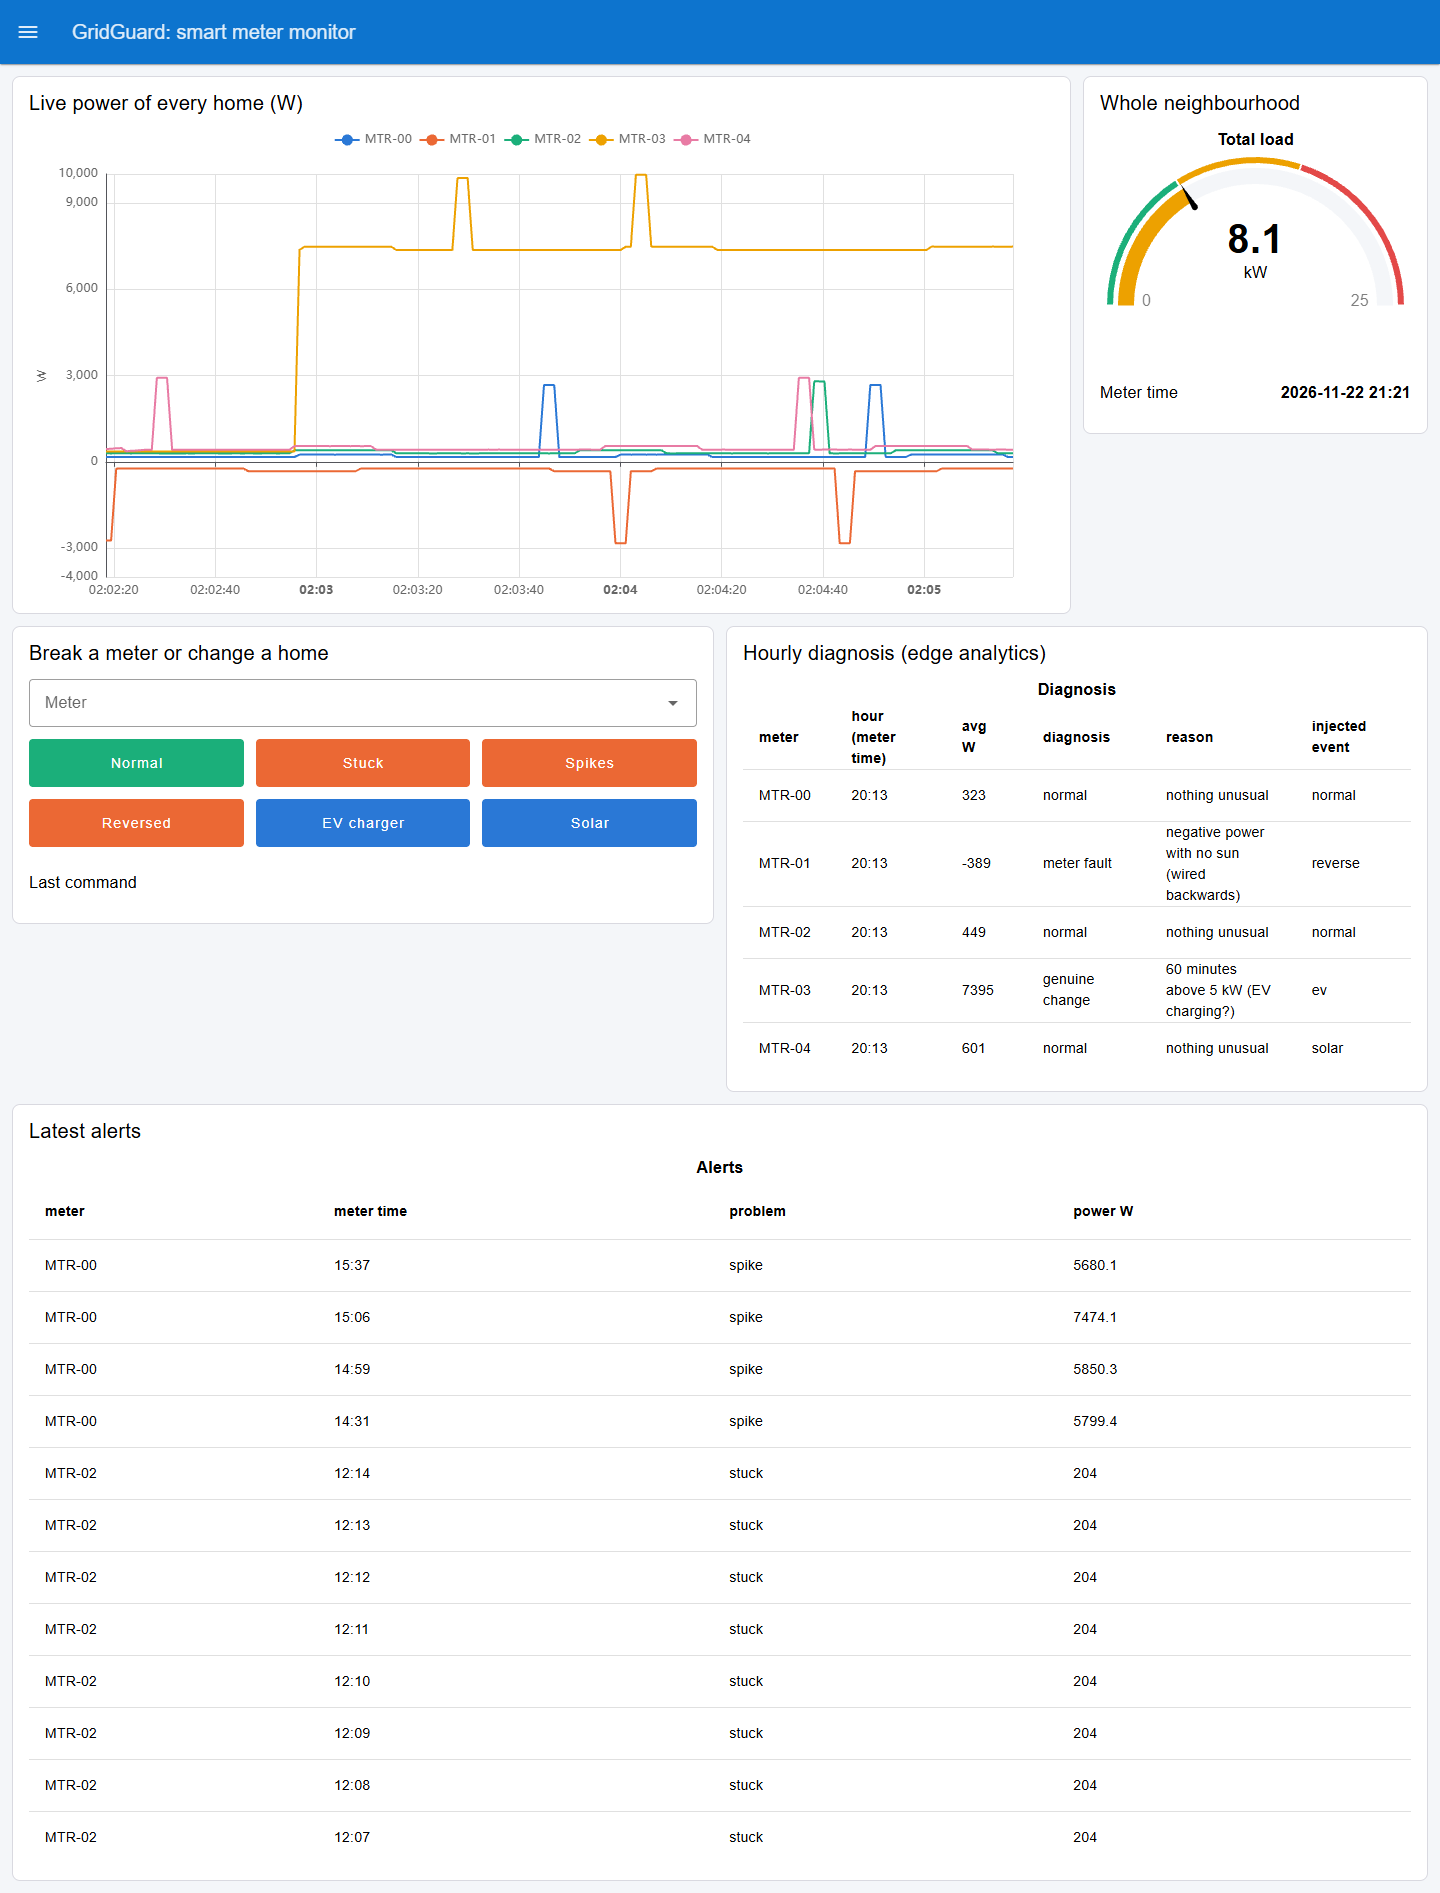
\includegraphics[width=0.9\textwidth]{dashboard-evening.png}
\caption{Dashboard in the evening: the EV charger on MTR-03 raises the total load, and the diagnosis reads \emph{genuine change}}
\label{fig:dash2}
\end{figure}

\subsection{Stored data}

For the recorded day, MongoDB holds 7,135 readings from five meters, 454 of them flagged, and 120 hourly diagnoses (5 meters $\times$ 24 hours). Three example documents follow.

\begin{lstlisting}[caption={A flagged reading, an alert and a diagnosis as stored in MongoDB}]
readings:  {"meter_id": "MTR-01", "household_id": "house-01",
            "session": "2026-11-22T20:13:48.295Z", "ts": "2026-11-22T00:20:00.000Z",
            "power_w": -170.9, "voltage_v": 228.6, "flags": ["reverse"],
            "received_at": "2026-11-22T20:14:09.481Z"}
alerts:    {"meter_id": "MTR-02", "session": "2026-11-22T20:13:48.295Z",
            "ts": "2026-11-22T08:25:00.000Z", "problem": "stuck", "power_w": 204}
diagnosis: {"meter_id": "MTR-03", "hour_start": "2026-11-22T19:13:00.000Z",
            "avg_w": 7638, "max_w": 9976, "min_w": 7357, "energy_kwh": 7.638,
            "frozen_share": 0, "spikes": 0, "negative_share": 0,
            "heavy_minutes": 60, "diagnosis": "genuine change",
            "reason": "60 minutes above 5 kW (EV charging?)"}
\end{lstlisting}

\subsection{Analysis of the recorded day (notebook 1)}

\begin{figure}[H]
\centering
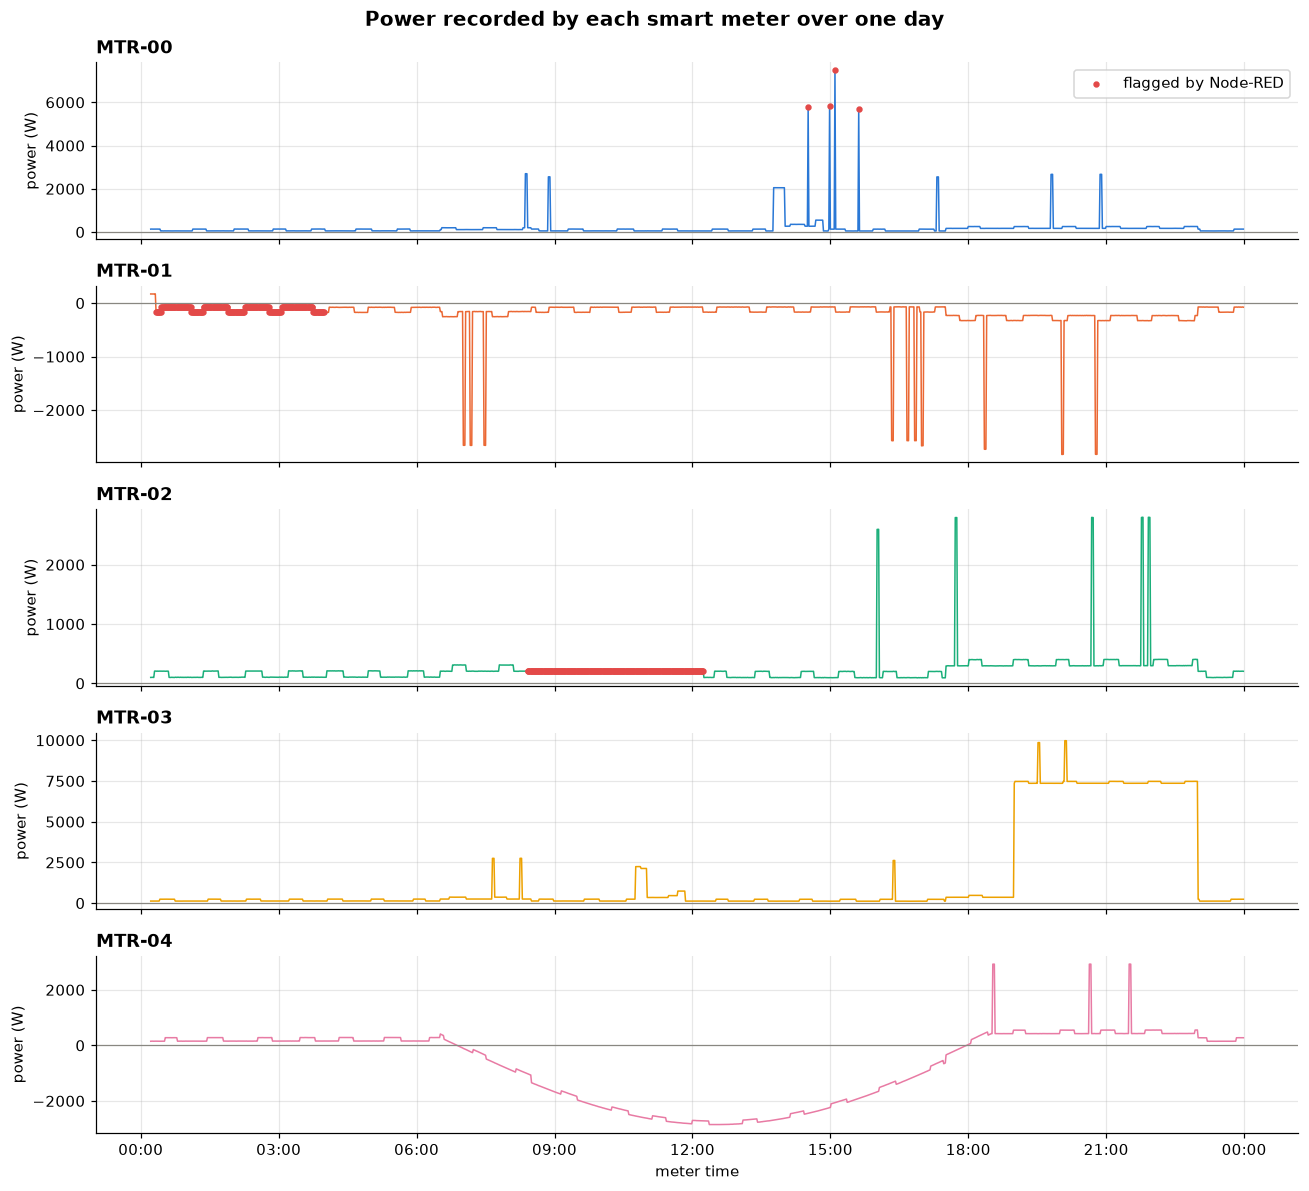
\includegraphics[width=0.92\textwidth]{nb1_day.png}
\caption{Power of every meter over the recorded day. Red dots are readings flagged by Node-RED.}
\label{fig:day}
\end{figure}

Figure~\ref{fig:day} shows each injected condition:
\begin{itemize}
\item MTR-00 has four isolated spikes in the afternoon;
\item MTR-01 stays below zero all day;
\item MTR-02 is flat from about 08:25 to 12:10;
\item MTR-03 draws more than 7~kW from 19:00 to 23:00;
\item MTR-04 dips to $-2.8$~kW around midday.
\end{itemize}

Normal kettle switch-ons (2.5--2.7~kW) were not flagged as spikes, because they stay below the 4~kW limit and last more than one minute. Table~\ref{tab:flags} counts the flags.

\begin{table}[H]
\centering
\caption{Readings flagged by Node-RED in the recorded day}
\label{tab:flags}
\small
\begin{tabular}{lcccc}
\toprule
\textbf{Meter} & \textbf{reverse} & \textbf{stuck} & \textbf{spike} & \textbf{Injected condition}\\
\midrule
MTR-00 & 0 & 0 & 4 & spikes 14:13--16:13 \\
MTR-01 & 220 & 0 & 0 & reversed all day \\
MTR-02 & 0 & 230 & 0 & stuck 08:13--12:13 \\
MTR-03 & 0 & 0 & 0 & EV charger (genuine) \\
MTR-04 & 0 & 0 & 0 & solar panels (genuine) \\
\bottomrule
\end{tabular}
\end{table}

\begin{figure}[H]
\centering
\begin{subfigure}{0.55\textwidth}\centering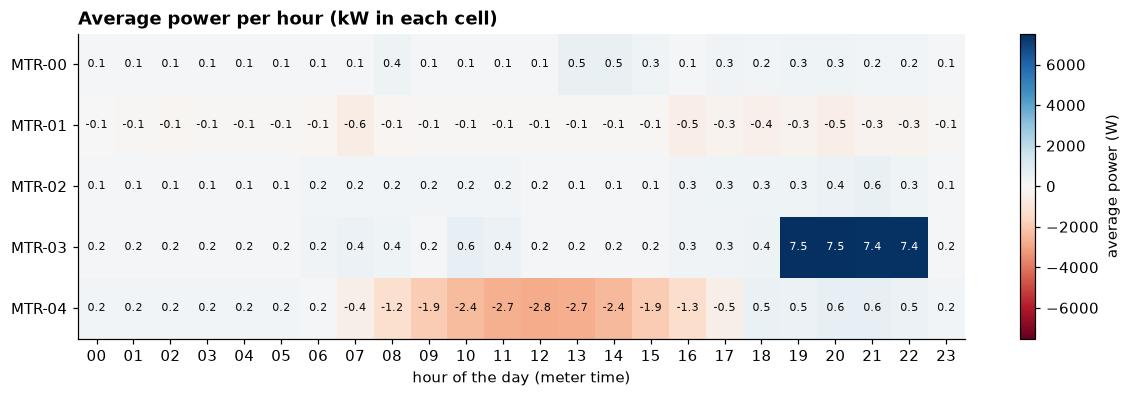
\includegraphics[width=\textwidth]{nb1_heatmap.png}\caption{Average power per hour (blue: drawing power, red: exporting)}\end{subfigure}\hfill
\begin{subfigure}{0.43\textwidth}\centering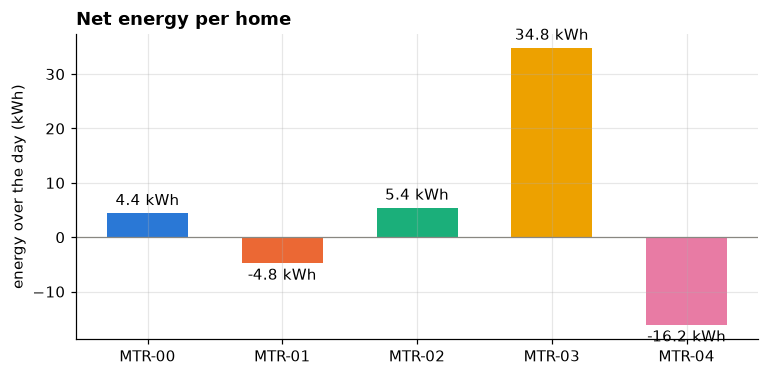
\includegraphics[width=\textwidth]{nb1_energy.png}\caption{Net energy per home}\end{subfigure}
\caption{Daily load profile and energy per home}
\label{fig:profile}
\end{figure}

In Figure~\ref{fig:profile}, the EV home uses the most energy: 34.8~kWh, against 4.4--5.4~kWh for a normal home. The solar home has a negative net energy of $-16.2$~kWh because of its daytime export. The reversed meter reports $-4.8$~kWh, which is impossible for a home without generation and is a strong sign of a wiring fault.

\begin{figure}[H]
\centering
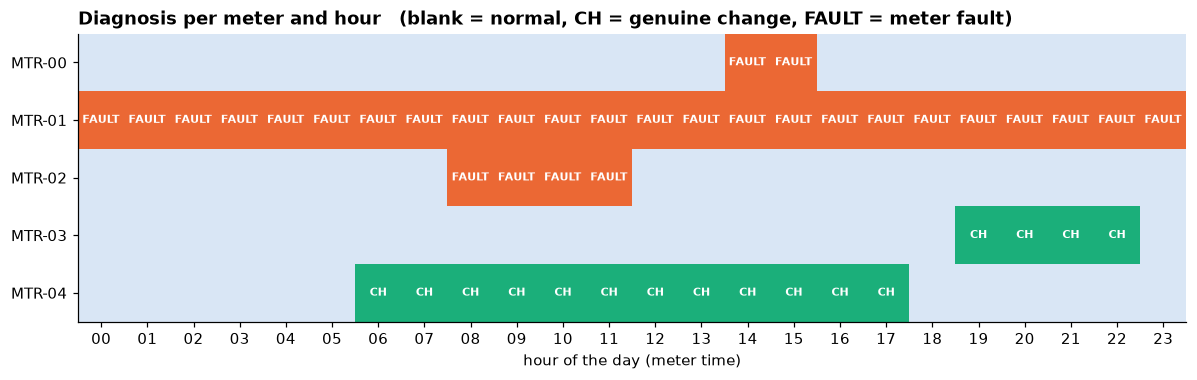
\includegraphics[width=\textwidth]{nb1_diagnosis.png}
\caption{Hourly diagnosis made by Node-RED for every meter}
\label{fig:diaggrid}
\end{figure}

\begin{table}[H]
\centering
\caption{Hourly diagnoses in the recorded day (24 hours per meter)}
\label{tab:diag}
\small
\begin{tabularx}{\textwidth}{lccc L}
\toprule
\textbf{Meter} & \textbf{normal} & \textbf{fault} & \textbf{change} & \textbf{Reason given}\\
\midrule
MTR-00 & 22 & 2 & 0 & impossible spikes \\
MTR-01 & 0 & 24 & 0 & wired backwards (night); negative day and night (day) \\
MTR-02 & 20 & 4 & 0 & reading frozen \\
MTR-03 & 20 & 0 & 4 & minutes above 5 kW (EV charging?) \\
MTR-04 & 12 & 0 & 12 & exporting in daylight (solar panels?) \\
\bottomrule
\end{tabularx}
\end{table}

\subsection{IoT test cases}

\begin{longtable}{>{\raggedright\arraybackslash}p{1.15cm} >{\raggedright\arraybackslash}p{3.25cm} >{\raggedright\arraybackslash}p{4.0cm} >{\raggedright\arraybackslash}p{4.0cm} >{\raggedright\arraybackslash}p{1.15cm}}
\caption{Test cases for the IoT pipeline}\label{tab:tc}\\
\toprule
\textbf{ID} & \textbf{Test} & \textbf{Expected} & \textbf{Observed} & \textbf{Result}\\
\midrule
\endfirsthead
\toprule
\textbf{ID} & \textbf{Test} & \textbf{Expected} & \textbf{Observed} & \textbf{Result}\\
\midrule
\endhead
TC-01 & Meter publishes over MQTT & Reading received and stored once per second & 7,135 readings stored for the day, all with session id & Pass \\
TC-02 & MTR-02 set to stuck & \texttt{stuck} flags after 10 equal readings; hourly \emph{meter fault: reading frozen} & 230 \texttt{stuck} flags; 4 fault hours (08--11) & Pass \\
TC-03 & MTR-00 set to spike & \texttt{spike} flags; \emph{meter fault: impossible spikes} & 4 \texttt{spike} flags, on the spike itself; 2 fault hours (14--15) & Pass \\
TC-04 & MTR-01 set to reverse & \texttt{reverse} flags at night; fault all day, never ``solar'' & 220 \texttt{reverse} flags (00--04); 24 of 24 hours \emph{meter fault} & Pass \\
TC-05 & MTR-04 set to solar & No fault; \emph{genuine change} in daylight & 0 flags; 12 hours \emph{exporting in daylight}; 0 fault hours & Pass \\
TC-06 & MTR-03 set to EV & No fault; \emph{genuine change} in the evening & 0 flags; 4 hours (19--22) \emph{genuine change} & Pass \\
TC-07 & Kettle switch-ons on normal meters & Not flagged & No flags on 2.5--2.7~kW kettle peaks & Pass \\
TC-08 & Dashboard button (Spikes on MTR-00) & Mode changes; spikes appear & Text ``MTR-00 is now: spike''; spikes appear in chart and alert table & Pass \\
TC-09 & MQTT command \texttt{\{"mode":} \texttt{"stuck"\}} sent to the control topic of MTR-02 & Mode changes & The recorded day was driven by such commands (TC-02 to TC-06) & Pass \\
TC-10 & Hourly diagnosis output & One document per meter per hour & 120 documents (5 $\times$ 24) & Pass \\
TC-11 & ThingSpeak with no key & Nothing sent; grey status & Status ``no THINGSPEAK\_WRITE\_KEY set'' & Pass \\
TC-12 & ThingSpeak with a wrong key & Request reaches ThingSpeak and is refused & Status ``ThingSpeak refused (400 / 0)'' & Pass \\
TC-13 & ThingSpeak with the channel's key & Status ``sent entry N''; charts fill & To be shown live with the team's channel key & -- \\
\bottomrule
\end{longtable}

\subsection{Federated learning results (notebook 2)}

\begin{figure}[H]
\centering
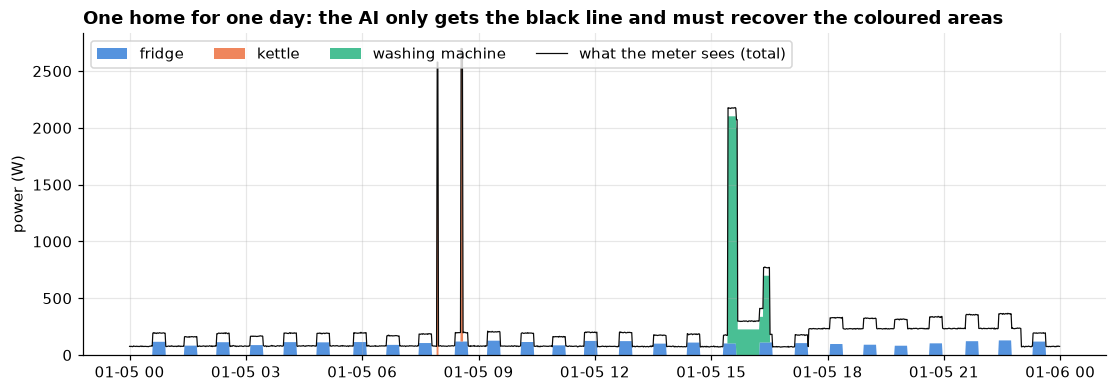
\includegraphics[width=\textwidth]{nb2_home.png}
\caption{One simulated home for one day: the model sees only the black total and must recover the coloured appliance areas}
\label{fig:home}
\end{figure}

\begin{figure}[H]
\centering
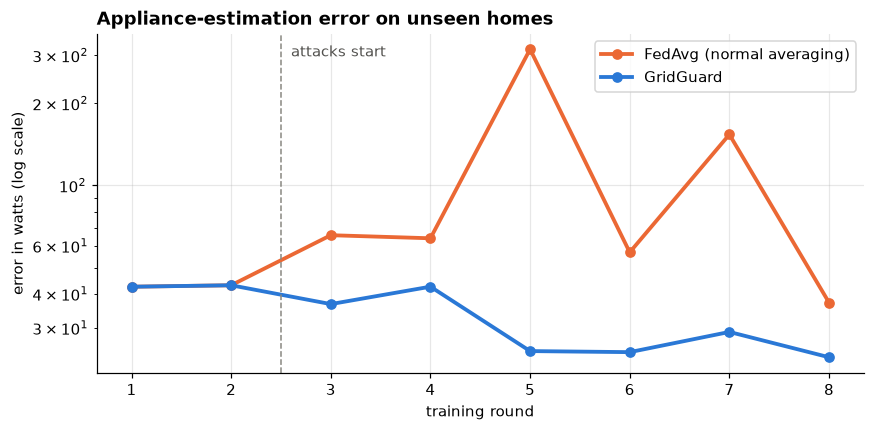
\includegraphics[width=0.8\textwidth]{nb2_error.png}
\caption{Appliance-estimation error on two unseen homes per round (log scale). Attacks start in round 3.}
\label{fig:err}
\end{figure}

\begin{table}[H]
\centering
\caption{Mean absolute error (W) on unseen homes after each round}
\label{tab:rounds}
\small
\begin{tabular}{lcccccccc}
\toprule
\textbf{Round} & 1 & 2 & 3 & 4 & 5 & 6 & 7 & 8\\
\midrule
FedAvg & 42.5 & 43.0 & 65.7 & 64.0 & 316.0 & 56.8 & 153.8 & 37.2 \\
GridGuard & 42.5 & 43.0 & 36.7 & 42.5 & 24.7 & 24.5 & 29.0 & \textbf{23.4} \\
\bottomrule
\end{tabular}
\end{table}

Both methods are identical in rounds 1 and 2, when every home is honest. As soon as the attacks start, FedAvg's error jumps and swings wildly, up to 316~W in round 5, the round in which the tampering attack also begins. GridGuard keeps improving and finishes 37\% lower than FedAvg.

\begin{figure}[H]
\centering
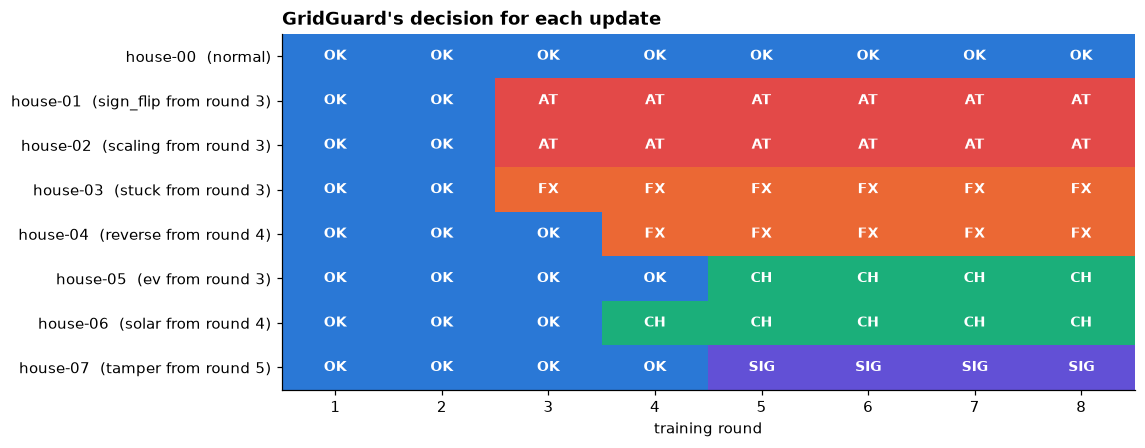
\includegraphics[width=\textwidth]{nb2_decisions.png}
\caption{GridGuard's decision for every home in every round. OK: benign; CH: genuine change (half weight); FX: meter fault (quarantined); AT: attack (rejected); SIG: bad signature (rejected).}
\label{fig:decisions}
\end{figure}

\begin{figure}[H]
\centering
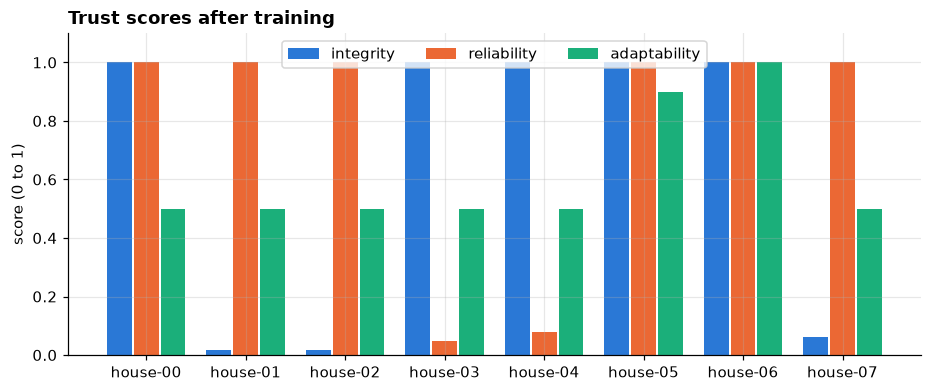
\includegraphics[width=0.85\textwidth]{nb2_trust.png}
\caption{Trust scores after training. Attackers lose integrity, faulty meters lose reliability but keep integrity, and the EV and solar homes gain adaptability.}
\label{fig:trust}
\end{figure}

\begin{table}[H]
\centering
\caption{GridGuard scorecard (64 decisions: 8 homes $\times$ 8 rounds)}
\label{tab:score}
\small
\begin{tabular}{lr}
\toprule
\textbf{Measure} & \textbf{Result}\\
\midrule
FedAvg final error & 37.2 W \\
GridGuard final error & 23.4 W \\
Causes identified correctly & 97\% \\
Attacks blocked & 100\% \\
Faulty meters quarantined & 100\% \\
Honest homes wrongly excluded & 0\% \\
Audit-chain edit detected & yes, at record 17 \\
\bottomrule
\end{tabular}
\end{table}

\begin{longtable}{>{\raggedright\arraybackslash}p{1.15cm} >{\raggedright\arraybackslash}p{3.4cm} >{\raggedright\arraybackslash}p{3.85cm} >{\raggedright\arraybackslash}p{3.85cm} >{\raggedright\arraybackslash}p{1.15cm}}
\caption{Test cases for the federated-learning part}\label{tab:fltc}\\
\toprule
\textbf{ID} & \textbf{Scenario} & \textbf{Expected} & \textbf{Observed} & \textbf{Result}\\
\midrule
\endfirsthead
\toprule
\textbf{ID} & \textbf{Scenario} & \textbf{Expected} & \textbf{Observed} & \textbf{Result}\\
\midrule
\endhead
FL-01 & house-01 sign flip ($-5\times$) from round 3 & Rejected as malicious & AT in rounds 3--8; integrity 1.0 $\to$ 0.02 & Pass \\
FL-02 & house-02 scaling ($20\times$) from round 3 & Rejected as malicious & AT in rounds 3--8 & Pass \\
FL-03 & house-07 update tampered after signing, from round 5 & Rejected by signature check & SIG in rounds 5--8 & Pass \\
FL-04 & house-03 stuck meter from round 3 & Quarantined, integrity kept & FX in rounds 3--8; reliability 0.05, integrity 1.0 & Pass \\
FL-05 & house-04 reversed meter from round 4 & Quarantined, not called solar & FX in rounds 4--8 & Pass \\
FL-06 & house-06 solar from round 4 & Accepted as genuine change & CH in rounds 4--8 & Pass \\
FL-07 & house-05 EV from round 3 & Accepted as genuine change & OK (accepted) in rounds 3--4, CH in rounds 5--8 & Partial \\
FL-08 & house-00 normal & Always accepted & OK in all 8 rounds & Pass \\
FL-09 & Edit one old decision in the audit log & Chain verification fails at that record & Record 17 changed from malicious to benign; check reports record 17 & Pass \\
\bottomrule
\end{longtable}

The two incorrect decisions (FL-07) are the EV home in rounds 3 and 4. It was labelled \emph{benign} instead of \emph{genuine change}. Its update was still accepted, so no honest data was lost; GridGuard simply recognised the change two rounds later. This accounts for the 3\% of causes not identified correctly.

\chapter{Conclusion \& Future Scope}

\section{Summary of Work and Achievements}

The project delivers a working IoT analytics pipeline built with Node-RED, MQTT, MongoDB and ThingSpeak, and a federated-learning study in Jupyter that implements the GridGuard idea from the synopsis.

\begin{itemize}
\item \textbf{Collection and transport:} five simulated smart meters publish over MQTT to a broker inside Node-RED; their condition can be changed live from the dashboard or by any MQTT client.
\item \textbf{Real-time analytics:} every reading is validated with four rules, and every meter-hour is diagnosed at the edge. In the recorded day all faults (reversed, stuck, spikes) were diagnosed as \emph{meter fault}, and the EV and solar homes as \emph{genuine change}, with no false alarms on normal appliance use.
\item \textbf{Storage and cloud:} readings, alerts and diagnoses are stored in MongoDB, and 20-second summaries are prepared for ThingSpeak.
\item \textbf{Visualisation:} a live Node-RED dashboard and two notebooks with nine analysis charts.
\item \textbf{Secure federated learning:} compared with FedAvg, GridGuard lowered the final error from 37.2~W to 23.4~W. It blocked all attacks, quarantined all faulty meters without lowering their owners' integrity, excluded no honest home, and detected both in-transit tampering and audit-log editing.
\end{itemize}

\textbf{Contribution of object-oriented concepts.} Object-oriented ideas appear throughout the system, although the IoT layer is event-driven rather than class-based:

\begin{itemize}
\item \textbf{Objects and messages.} Node-RED is built from node objects that exchange message objects (\texttt{msg} with a \texttt{payload}). Every reading, alert and diagnosis is a self-describing object, which is also why MongoDB can store it without a fixed schema.
\item \textbf{Encapsulation.} Each function node keeps its own private state in its context:
  \begin{itemize}
  \item the simulator keeps one \emph{home} object per meter (fridge state, held value, and so on);
  \item \emph{Check reading} keeps a \texttt{\{before, pending, repeats\}} object per meter;
  \item \emph{Hourly diagnosis} keeps a 60-reading buffer per meter.
  \end{itemize}
  Other nodes cannot change this state; they interact only through messages. In Python, \texttt{AuditChain} hides its list of records behind two methods, \texttt{add()} and \texttt{first\_broken()}.
\item \textbf{Inheritance and polymorphism.} \texttt{Seq2Point} inherits from \texttt{torch.nn.Module} and overrides \texttt{forward()}. PyTorch's training code, the optimiser and the loss work with it through the common \texttt{Module} interface (\texttt{model(x)}, \texttt{parameters()}) without knowing the concrete class. The same class is instantiated by every home and by the server.
\item \textbf{Abstraction and reuse.} One MQTT broker configuration node is shared by three MQTT nodes, and one MongoDB client configuration by three database nodes, just as several objects can share one instance. MQTT topics hide which device produced a message, so a real meter could replace the simulator without any change to the rest of the flow.
\end{itemize}

These concepts made the system modular: each part can be understood, tested and replaced on its own. Most of the analytics logic itself, however, is written as short procedural functions. That suits rule-based stream processing, but means OOP is a supporting rather than a central technique in this project.

\section{Impact on society, Environmental sustainability, Ethical issues and compliance}

\textbf{Society.}
\begin{itemize}
\item Separating meter faults from attacks protects households from being blamed, or cut off, for a hardware problem.
\item Early detection of stuck or reversed meters prevents wrong bills and long disputes.
\item Appliance-level feedback from NILM helps families understand and reduce their consumption.
\end{itemize}

\textbf{Environmental sustainability.}
\begin{itemize}
\item Recognising rooftop solar export and EV charging as legitimate behaviour supports their adoption instead of penalising it.
\item Neighbourhood load data (the ThingSpeak total-load field) helps utilities plan for evening EV peaks.
\item The edge analytics are lightweight rules that run on modest hardware, and only summaries go to the cloud, which saves bandwidth and energy.
\end{itemize}

\textbf{Ethical issues and compliance.}
\begin{itemize}
\item \textbf{Privacy.} Minute-level consumption data reveals when people are at home, when they sleep and which appliances they own. GridGuard keeps raw readings inside the home in the federated setting and sends only model updates and six summary numbers. The ThingSpeak channel receives only 20-second averages. A real deployment in India would have to follow the Digital Personal Data Protection Act, 2023: purpose limitation, consent and data minimisation.
\item \textbf{Fairness and transparency.} Automatic decisions about a household must be explainable and contestable. Every diagnosis is stored with a human-readable reason, and every federated decision is recorded in a tamper-evident audit chain.
\item \textbf{Uncertainty.} When the evidence is mixed, GridGuard holds the update back (\emph{uncertain}) instead of accusing the home of an attack.
\item \textbf{Security of credentials.} The ThingSpeak Write API key is stored in a Node-RED environment variable and must not be published in a public repository.
\item \textbf{Data used.} This project uses only simulated data, so no real person's consumption was collected.
\end{itemize}

\section{Limitations of the Work and Future Scope}

\textbf{Limitations.}
\begin{itemize}
\item The meters are simulated. Real meters have more noise, communication gaps and appliance types, and the thresholds (4~kW spikes, 10 equal readings, sun hours from 06:00 to 19:00) would need tuning, and seasonal adjustment of the sun hours, for real data.
\item The edge rules are fixed. A home with a battery that discharges at night could look like a reversed meter, and a large heat pump could look like an EV.
\item The federated experiment uses eight simulated homes in one notebook rather than separate devices on a network, and it does not use the public datasets named in the synopsis.
\item Label/model poisoning, gradual meter drift, macro-F1 scores, verification latency and Raspberry Pi resource usage, all listed in the synopsis, were not evaluated.
\item In the experiment the EV home's change was recognised two rounds late (FL-07).
\item The ThingSpeak upload was verified up to the point where ThingSpeak answers; it still has to be demonstrated with the team's own channel key.
\end{itemize}

\textbf{Future scope.}
\begin{itemize}
\item Connect real meters or energy-monitoring plugs (for example an ESP32 with a current sensor) to the same MQTT topics; the rest of the flow needs no change.
\item Run the Node-RED edge logic on a Raspberry Pi and measure CPU, memory and power, as planned in the synopsis.
\item Evaluate the federated part on REDD, UK-DALE and REFIT, use the Flower framework with clients on separate machines, and report macro-F1 and verification latency.
\item Replace the fixed thresholds with learned per-home baselines, and add weather or sunrise data so the solar rule adapts to the season.
\item Add gradual drift and label poisoning to the test scenarios, and allow homes with batteries.
\item Move the database and the federated server to a managed cloud (for example MongoDB Atlas or AWS) and secure MQTT with TLS and per-device credentials.
\end{itemize}

\begin{thebibliography}{99}
\addcontentsline{toc}{chapter}{References}
\bibitem{hart} G. W. Hart, ``Nonintrusive appliance load monitoring,'' \emph{Proceedings of the IEEE}, vol. 80, no. 12, pp. 1870--1891, Dec. 1992.
\bibitem{s2p} C. Zhang, M. Zhong, Z. Wang, N. Goddard, and C. Sutton, ``Sequence-to-point learning with neural networks for non-intrusive load monitoring,'' in \emph{Proc. AAAI Conference on Artificial Intelligence}, 2018, pp. 2604--2611.
\bibitem{fedavg} B. McMahan, E. Moore, D. Ramage, S. Hampson, and B. A. y Arcas, ``Communication-efficient learning of deep networks from decentralized data,'' in \emph{Proc. 20th Int. Conf. Artificial Intelligence and Statistics (AISTATS)}, 2017, pp. 1273--1282.
\bibitem{mqtt} OASIS, ``MQTT Version 5.0,'' OASIS Standard, Mar. 2019. [Online]. Available: \url{https://docs.oasis-open.org/mqtt/mqtt/v5.0/mqtt-v5.0.html}
\bibitem{nodered} OpenJS Foundation, ``Node-RED documentation.'' [Online]. Available: \url{https://nodered.org/docs/}
\bibitem{mongodb} MongoDB, Inc., ``MongoDB manual.'' [Online]. Available: \url{https://www.mongodb.com/docs/manual/}
\bibitem{thingspeak} The MathWorks, Inc., ``ThingSpeak documentation.'' [Online]. Available: \url{https://www.mathworks.com/help/thingspeak/}
\bibitem{krum} P. Blanchard, E. M. El Mhamdi, R. Guerraoui, and J. Stainer, ``Machine learning with adversaries: Byzantine tolerant gradient descent,'' in \emph{Advances in Neural Information Processing Systems (NeurIPS)}, 2017, pp. 119--129.
\bibitem{trimmed} D. Yin, Y. Chen, K. Ramchandran, and P. Bartlett, ``Byzantine-robust distributed learning: Towards optimal statistical rates,'' in \emph{Proc. 35th Int. Conf. Machine Learning (ICML)}, 2018, pp. 5650--5659.
\bibitem{fltrust} X. Cao, M. Fang, J. Liu, and N. Z. Gong, ``FLTrust: Byzantine-robust federated learning via trust bootstrapping,'' in \emph{Proc. Network and Distributed System Security Symposium (NDSS)}, 2021.
\bibitem{ed25519} D. J. Bernstein, N. Duif, T. Lange, P. Schwabe, and B.-Y. Yang, ``High-speed high-security signatures,'' \emph{Journal of Cryptographic Engineering}, vol. 2, no. 2, pp. 77--89, 2012.
\bibitem{sha} National Institute of Standards and Technology, ``Secure Hash Standard (SHS),'' FIPS PUB 180-4, Aug. 2015.
\bibitem{haber} S. Haber and W. S. Stornetta, ``How to time-stamp a digital document,'' \emph{Journal of Cryptology}, vol. 3, no. 2, pp. 99--111, 1991.
\bibitem{ukdale} J. Kelly and W. Knottenbelt, ``The UK-DALE dataset, domestic appliance-level electricity demand and whole-house demand from five UK homes,'' \emph{Scientific Data}, vol. 2, art. 150007, 2015.
\bibitem{redd} J. Z. Kolter and M. J. Johnson, ``REDD: A public data set for energy disaggregation research,'' in \emph{Proc. SustKDD Workshop on Data Mining Applications in Sustainability}, 2011.
\bibitem{refit} D. Murray, L. Stankovic, and V. Stankovic, ``An electrical load measurements dataset of United Kingdom households from a two-year longitudinal study,'' \emph{Scientific Data}, vol. 4, art. 160122, 2017.
\bibitem{pytorch} A. Paszke \emph{et al.}, ``PyTorch: An imperative style, high-performance deep learning library,'' in \emph{Advances in Neural Information Processing Systems (NeurIPS)}, 2019, pp. 8024--8035.
\bibitem{dashboard} FlowFuse, ``Node-RED Dashboard 2.0 documentation.'' [Online]. Available: \url{https://dashboard.flowfuse.com/}
\end{thebibliography}

\chapter*{Appendix}
\addcontentsline{toc}{chapter}{Appendix}

\section*{Team Roles and Contributions}

\textbf{Mukul Aggarwal (2401030239):} Node-RED flows: meter simulator, MQTT broker and topics, \emph{Check reading} and \emph{Hourly diagnosis} logic, MongoDB storage, live dashboard; recording and testing of the simulated day.

\vspace{4pt}
\textbf{Shivam Diwaker (2401030245):} ThingSpeak channel and upload flow; notebook 1 (data analysis and charts); notebook 2 (Seq2Point model, FedAvg baseline, GridGuard evidence, trust, signatures and audit chain); documentation and report.

\section*{How to Run the Project}

\begin{enumerate}
\item Start MongoDB (Windows service) so that it listens on \texttt{localhost:27017}.
\item In the \texttt{node-red} folder run \texttt{npm install} once, then \texttt{npm start}.
\item Open \url{http://localhost:1880} for the flows and \url{http://localhost:1880/dashboard} for the dashboard.
\item Optional: in tab 3, set \texttt{THINGSPEAK\_WRITE\_KEY} to the channel's Write API key and press \emph{Deploy}.
\item For the notebooks: create a Python virtual environment, run \texttt{pip install} \texttt{-r requirements.txt}, and then open the notebooks in Jupyter or VS Code. Both are saved with their outputs.
\end{enumerate}

\end{document}
